\chapter{Digital Electronics}
Digital electronics is essential to understanding the design and working of a wide range of applications. Digital systems contain devices that process the physical
quantities represented in digital form.
\section{Number system}
Number System is a way to represent the numbers in the computer architecture. There are four different types of the number system, 
\begin{enumerate}
	\item Decimal number sysytem(Base 10)
	\item Binary number system (base 2)
	\item Octal number system(base 8)
	\item Hexadecimal number system (base 16)
\end{enumerate}

\subsection{Decimal number system}
In the decimal number system, is the radix-10 number system and therefore has 10 different digits or symbols. These are $0,1,2,3,4,5,6,7,8,9$. Each digit in the decimal system has a position and every digit is ten times more significant than the previous digit. Suppose, 25 is a decimal number, then 2 is ten times more than 5 . 
The place values of different digits in a mixed decimal number, starting from the decimal point, are $10^{0}, 10^{1}, 10^{2}$ and so on (for the integer part) and $10^{-1}, 10^{-2}, 10^{-3}$ and so on (for the fractional part). The value or magnitude of a given decimal number can be expressed as the sum of the various digits multiplied by their place values or weights.
\begin{example}
	\begin{align*}
	(92)_{10}&=9 \times 10^{1}+2 \times 10^{0} \\
	(200)_{10}&=2 \times 10^{2}+0 \times 10^{1}+0 \times 10^{0}\\
	(30.2)_{10}&=3 \times 10^{1}+0 \times 10^{0}+2 \times 10^{-1} \\
	(212.367)_{10}&=2 \times 10^{2}+1 \times 10^{1}+2 \times 10^{0}+3 \times 10^{-1}+6 \times 10^{-2}+7 \times 10^{-3}
	\end{align*}
\end{example}

\subsection{Binary number system}
The binary number system is a radix-2 number system with ‘0’ and ‘1’ as the two independent digits. Starting from the binary point, the place values of different digits in a mixed binary number are $2^{0}, 2^{1}, 2^{2}$ and so on (for the integer part) and $2^{-1}, 2^{-2}, 2^{-3}$ and so on (for the fractional part). The binary system is applied internally by almost all latest computers and computer-based devices because of it's direct implementation in electronic circuits using logic gates. Every digit is referred to as a bit.
\begin{example}
	10101 is a five-bit binary number, 101 is a three-bit binary number,100001 is a six-bit binary number
\end{example}


\colorlet{ocre1}{ocre!70!}
\colorlet{ocrel}{ocre!30!}
\setlength\arrayrulewidth{1pt}
\begin{table}[H]
	\centering
	\arrayrulecolor{ocre}
	\begin{tabular}{|p{1.5cm}|p{2cm}||p{1.5cm}|p{2cm}|}
		\hline
		\multicolumn{4}{|c|}{\textbf{Binary numbers}}\\\hline\hline
		\rowcolor{ocrel}Decimal Number&Binary Equivalent &Decimal Number&Binary Equivalent \\\hline
		\hline 1 & 1 & 11 & 1011 \\
		\hline 2 & 10 & 12 & 1100 \\
		\hline 3 & 11 & 13 & 1101 \\
		\hline 4 & 100 & 14 & 1110 \\
		\hline 5 & 101 & 15 & 1111 \\
		\hline 6 & 110 & 16 & 10000 \\
		\hline 7 & 111 & 17 & 10001 \\
		\hline 8 & 1000 & 18 & 10010 \\
		\hline 9 & 1001 & 19 & 10011 \\
		\hline 10 & 1010 & 20 & 10100 \\
		\hline
	\end{tabular}
	\caption{Table of binary numbers}
\end{table}

\subsection{Decimal to binary conversion}
Decimal to binary conversion is done by a method called double which is more popular for decimal to binary conversion in this method integers and fractions are handled seperately. Here the decimal numner is repeatdly divided by 2 and reminder after each division is taken in the reverse order. 
\begin{exercise}
	Convert the decimal number 25 into binary .\\\\
	$\begin{array}{ccc}\text { Divisor } & \text { Dividend } & \text { Remainder } \\  2 & 25 & - \\ 2 & 12 & 1 \\ 2 & 6 & 0 \\ 2 & 3 & 0 \\ 2 & 1 & 1  \\ - & 0 & 1\end{array}$\qquad
	$(25)_{10}=(11001)_{2}$
\end{exercise}

\begin{exercise}
	Convert the decimal number 125 into binary .\\\\
	$\begin{array}{ccc}\text { Divisor } & \text { Dividend } & \text { Remainder } \\  2 & 125 & - \\ 2 & 62 & 1 \\ 2 &31& 0 \\ 2 & 15 & 1 \\ 2 & 7 & 1  \\ 2 & 3 & 1 \\ 2 & 1 & 1 \\ - & 0 & 1\end{array}$\qquad
	$(125)_{10}=(1111101)_{2}$
\end{exercise}
\begin{exercise}
	Convert the decimal number 68 into binary .\\\\
	$\begin{array}{ccc}\text { Divisor } & \text { Dividend } & \text { Remainder } \\  2 & 68 & - \\ 2 & 34 & 0 \\ 2 & 17 & 0 \\ 2 & 8 & 1 \\ 2 & 4 & 0  \\ 2 & 2 & 0 \\ 2 & 1 & 0 \\ - & 0 & 1\end{array}$\qquad
	$(68)_{10}=(1000100)_{2}$
\end{exercise}

\subsubsection{Conversion of decimal fraction to binary 
	fraction}
Instead of division, multiplication by 2 is carried out and the integer part of the result is saved and placed after the decimal point. The fractional part is again multiplied by 2 and the process repeated.
\begin{exercise}
	Convert $(0.375)_{10}$ to binary fraction.
	\begin{align*}
	\text{The fractional part } &=0.375\\
	0.375 \times 2&=0.75 \hspace{0.2cm} \text{with a carry of  0}\\
	0.75 \times 2&=0.5 \hspace{0.4cm} \text{with a carry of  1}\\
	0.5 \times 2&=0 \hspace{0.7cm} \text{with a carry of  1}\\
	\text{The binary equivalent of } (0.375)_{10}&=(.011)_{2}
	\end{align*}
\end{exercise}
\begin{exercise}
	Convert $( 0.68)_{10}$ to binary fraction.
	\begin{align*}
	\text{The fractional part } &=0.68\\
	0.68 \times  2&=1.36  \hspace{0.2cm} \text{with a carry of  1}\\
	0.36 \times 2&=0.72  \hspace{0.2cm} \text{with a carry of  0}\\
	0.72 \times 2&=1.44  \hspace{0.2cm} \text{with a carry of  1}\\
	0.44 \times 2&=0.88  \hspace{0.2cm} \text{with a carry of  0}\\
	\text{The binary equivalent of } (0.68)_{10}&=0.1010 \ldots .
	&	\end{align*}
\end{exercise}
\begin{exercise}
	Convert the decimal number $7\frac{5}{8}$ into binary 
\end{exercise}
\begin{answer}
	$7\frac{5}{8}$ is written as $7.625$\\
	The binary number of the integer part 7 is 111. The decimal fraction 0.625 can be converted in to binary as before.\\
	\begin{align*}
	\begin{array}{lll}
	0.625\times2&=1.250&\text{carry}=1\\
	0.250\times2&=0.5&\text{carry}=0\\
	0.5\times2&=1.0&\text{carry}=1\\
	\therefore\left(7\frac{5}{8}\right) &=\left(111.101\right) _2\\
	\end{array}\\
	\end{align*}
\end{answer}

\begin{exercise}
	Convert $\frac{1}{5}=0.2$ in to binary.
\end{exercise}
\begin{answer}
	\begin{align*}
	\begin{array}{lll}
	0.2\times2=0.4&\quad\text{carry}&0\\
	0.4\times2=0.8&\quad\text{carry}&0\\
	0.8\times2=1.6&\quad\text{carry}&1\\
	0.6\times2=1.2&\quad\text{carry}&1\\
	0.2\times2=1.4&\quad\text{carry}&0\\
	0.4\times2=0.8&\quad\text{carry}&0\\
	0.8\times2=1.6&\quad\text{carry}&1\\
	0.6\times2=1.2&\quad\text{carry}&1\\
	\end{array}\\
	\end{align*}
	The binary fractions is 0.00110011.....it never terminate.
\end{answer}
\subsection{Binary to Decimal Conversion}
11011001 to decimal

$$
\begin{aligned}
&1 \times 2^{0} =1 \times 1=1 \\
&0 \times 2^{1} =0 \times 2=0\\
&0 \times 2^{2}=0 \times 4=0\\
&1 \times 2^{3}=1 \times 8=8\\
&1 \times 2^{4}=1 \times 16=16\\
&0 \times 2^{5}=0 \times 32=0\\
&1 \times 2^{6}=1 \times 64=64\\
&1 \times 2^{7}=1 \times 128=128\\
&1+8+16+64+128=217\\
&(11011001)_{2}=(217)_{10}
\end{aligned}
$$
\begin{exercise}
	Convert 1101.1001 into decimal. According to the positional weight 1101.1001 can be written as
\end{exercise}
\begin{answer}
	\begin{align*}
	1101.1001&=1\times2^3+1\times2^2+0\times2^1+2^0\\
	&+1\times2^{-1}+0\times2^{-2}+0\times2^{-3}+1\times2^{-4}\\
	&=8+4+0+1+\frac{1}{2}+0+0+\frac{1}{16}\\
	&=13\frac{9}{16}\quad \text{or}\quad13.5625
	\end{align*}
\end{answer}
\begin{exercise}
	Convert the binary number 1011.11 into decimal.
\end{exercise}
\begin{answer}
	\begin{align*}
	1011.11&=1\times2^3+0\times2^2+1\times2^1+1\times2^0\\
	&+1\times2^{-1}+1\times2^{-2}\\
	&=11+0.5+0.25=11.75
	\end{align*}
\end{answer}
\subsection{Binary addition}
Adding two binary numbers will give us a binary number itself. It is the simplest method. Addition of two single digit binary number is given in the table below.\\
$$\begin{tabular}{|l|l|l|}
\hline Binary Numbers & Addition & \\
\hline 0 & 0 & 0 \\
\hline 0 & 1 & 1 \\
\hline 1 & 0 & 1 \\
\hline 1 & 1 & $0 ;$ Carry $\rightarrow 1$ \\
\hline
\end{tabular}$$

\begin{exercise}
	Add the binary numbers 1110 and 1011
\end{exercise}
\begin{answer}
	\begin{align*}
	\begin{tabular}{ccccc}
	1&1&1&\text{carry}& \\
	&1&1&1&0\\
	+&1&0&1&1\\
	\hline 1&1&0&0&1
	\end{tabular}
	\end{align*}
\end{answer}
\begin{exercise}
	Add $8 \frac{1}{4}$ and $6 \frac{3}{4}$ in binary\\
\end{exercise}
\begin{answer}
	\begin{align*}
	\begin{tabular}{ccccccc}
	& & &1& &1&\text{carry}\\
	1&0&0&0&.&0&1\\
	&1&1&0&.&1&1\\
	\hline 1&1&1&1&.&0&0
	\end{tabular}
	\end{align*}
	\begin{align*}
	8 \frac{1}{4}&=8.25=1000.01_{2}\\
	6 \frac{3}{4}&=6.75=110.11_{2}\\
	8.25+6.75&=15\\
	\text{Answer is }&=(1111.00)_2
	\end{align*}
\end{answer}
\subsection{Binary substraction}
Subtracting two binary numbers will give us a binary number itself. It is also a straightforward method. Subtraction of two single-digit binary number is given in the table below.\\
$$\begin{tabular}{|l|l|l|}
\hline Binary Numbers & Subtraction&  \\
\hline 0 & 0 & 0 \\
\hline 0 & 1 & $1 ;$ Borrow 1 \\
\hline 1 & 0 & 1 \\
\hline 1 & 1 & 0 \\
\hline
\end{tabular}$$

\begin{exercise}
	Subtract 6 from 12 in binary system.
\end{exercise}
\begin{answer}
	\begin{align*}
	\intertext{Number Systems}
	(6)_{10}&=(110)_{2} ;(12)_{10}=(1100)_{2}\\
	\begin{tabular}{ccccc}
	&1&1&0&0\\
	--& &1&1&0\\
	\cline{2-5} & &1&1&0
	\end{tabular}
	\end{align*}
\end{answer}
\begin{exercise}
	Subtract 15 from 25 in the binary system
\end{exercise}
\begin{answer}
	\begin{align*}
	(15)_{10}&=(1111)_{2} ; \quad(25)_{10}=(11001)_{2}\\
	\begin{tabular}{cccccc}
	&1&1&0&0&1\\
	--& &1&1&1&1\\
	\cline{2-6} & &1&0&1&0
	\end{tabular}
	\end{align*}
\end{answer}
\begin{exercise}
	Subtract $\left(9 \frac{1}{2}\right)_{10}$ from $13 \frac{3}{4}$
\end{exercise}
\begin{answer}
	\begin{align*}
	9 \frac{1}{2}_{10}&=1001.1_{2} ; 13 \frac{3}{4}_{10}=1101.11_{2}\\
	\begin{tabular}{cccccccc}
	&1&1&0&1&.&1&1\\
	--&1&0&0&1&.&1& \\
	\cline{2-8} & &1&0&0&.&0&1
	\end{tabular}
	\end{align*}
\end{answer}
In the octal number system, we have the 7's and 8's complements. The 7's complement of a given octal number is obtained by subtracting each octal digit from 7 . For example, the 7 's complement of $(562)_{8}$ would be $(215)_{8}$. The 8 's complement is obtained by adding ' 1 ' to the 7 's complement. The 8 's complement of $(562)_{8}$ would be $(216)_{8}$
1.7.4 Hexadecimal Number System
The 15's and 16's complements are defined with respect to the hexadecimal number system. The 15's complement is obtained by subtracting each hex digit from 15. For example, the 15 's complement of $(3 \mathrm{BF})_{16}$ would be $(\mathrm{C} 40)_{16}$. The 16's complement is obtained by adding ' 1 ' to the 15 's complement. The 16's complement of $(2 \mathrm{AE})_{16}$ would be (D52) $)_{16}$.
\section{Octal number system}
The octal number system has a radix of 8 and therefore has eight distinct digits. The independent digits are 0,1 , $2,3,4,5,6$, and 7 . The next ten numbers that follow 7 , for example, would be $10,11,12,13,14,15,16,17,20$ and 21 . In fact, if we omit all the numbers containing the digits 8 or 9 or both from the decimal number system, we end up with octal number system. The place values for different digits in the octal number system are $8^{0}, 8^{1}$, $8^{2}$ and so on (for the integer part) and $8^{-1}, 8^{-2}, 8^{-3}$ and so on (for the fractional part). 

$$\begin{array}{|c|c|}
\hline \text { Octal Number } & \text { Binary Equivalent } \\
\hline 0 & 000 \\
\hline 1 & 001 \\
\hline 2 & 010 \\
\hline 3 & 011 \\
\hline 4 & 100 \\
\hline 5 & 101 \\
\hline 6 & 110 \\
\hline 7 & 111 \\
\hline
\end{array}$$



\subsubsection{Decimal to Octal number}
To convert decimal to octal number, octal dabble method is used. In this method, the decimal number is divided by 8 each time, it yields or gives a remainder. The first remainder we get is the Least Significant digit(LSD) and the last remainder is the Most  Significant Digit (MSD). Let us understand the conversion with the help example.

\begin{exercise}
	Suppose 560  is a decimal number. Convert it into an octal number.\\\\
	$\begin{array}{ccc}\text { Divisor } & \text { Dividend } & \text { Remainder } \\  8 & 560 & - \\ 8 & 70 & 0 \\ 8 & 8 & 6 \\ 8 & 1 & 0 \\ - & 1 & 1  \end{array}$\qquad
	$(560)_{10}=(1060)_{8}$
\end{exercise}

\begin{exercise}
	Convert 0.52 into an octal number.
\end{exercise}
\begin{answer}
	The fraction part of the decimal number has to be multiplied by 8 .\\
	$0.52 \times 8=0.16$ with carry 4\\
	$0.16 \times 8=0.28$ with carry 1\\
	$0.28 \times 8=0.24$ with carry 2\\
	$0.24 \times 8=0.92$ with carry 1\\
	So, for the fractional octal number, we read the generated carry from up to down.
	Therefore, 4121 is the octal number.	
\end{answer}
\subsubsection{Octal to Decimal}
To convert an octal number to decimal number we need to multiply each digit of the given octal with the reducing power of 8 .
\begin{exercise}
	Suppose$215_{8}$ is an octal number, then it's decimal form will be?
\end{exercise}
\begin{answer}
	$$
	\begin{aligned}
	215_{8} &=2 \times 8^{2}+1 \times 8^{1}+5 \times 8^{0} \\
	&=2 \times 64+1 \times 8+5 \times 1=128+8+5 \\
	&=141_{10}
	\end{aligned}
	$$	
\end{answer}
\section{Hexadecimal number system}
The hexadecimal number system is a radix- 16 number system and its 16 basic digits are $0,1,2,3,4,5,6,7,8$, $9, \mathrm{~A}, \mathrm{~B}, \mathrm{C}, \mathrm{D}, \mathrm{E}$, and $\mathrm{F}$. The place values or weights of different digits in a mixed hexadecimal number are $16^{0}$, $16^{1}, 16^{2}$ and so on (for the integer part) and $16^{-1}, 16^{-2}$, $16^{-3}$ and so on (for the fractional part). The decimal equivalent of $\mathrm{A}, \mathrm{B}, \mathrm{C}, \mathrm{D}, \mathrm{E}$ and $\mathrm{F}$ are $10,11,12,13,14$ and 15 , respectively, for obvious reasons. Hexadecimal number system provides a condensed way of representing large binary numbers stored and processed inside the computer. 
\renewcommand*{\arraystretch}{1.2}
$$\begin{aligned}
&\begin{array}{|c|c|}
\hline \text { hexadecimal } & \begin{array}{c}
\text { Binary representation of } \\
\text { Hexadecimal number }
\end{array} \\
\hline 0 & 0000 \\
1 & 0001 \\
2 & 0010 \\
3 & 0011 \\
4 & 0100 \\
5 & 0101 \\
6 & 0110 \\
7 & 0111 \\
8 & 1000 \\
9 & 1001 \\
\text { A } & 1010 \\
\text { B } & 1100 \\
\text { C } & 1101 \\
\text { D } & 1101 \\
\text { E } & 1110 \\
\text { F } & 1111 \\
\hline
\end{array}
\end{aligned}$$
\subsubsection{Decimal to hexadecimal}
\begin{exercise}
	Convert the decimal number 325 into hexadecimal\\\\
	$\begin{array}{ccc}\text { Divisor } & \text { Dividend } & \text { Remainder } \\  16 & 325 & - \\ 16 & 20 & 5 \\ 16 & 1 & 4 \\  - & 1 & 1  \end{array}$\qquad
	$(325)_{10}=(145)_{16}$
\end{exercise}
\begin{exercise}
	Convert the decimal number 58 into hexadecimal\\\\
	$\begin{array}{ccc}\text { Divisor } & \text { Dividend } & \text { Remainder } \\  16 & 58 & - \\ 16 & 3 & A \\ - & 3 & 3  \end{array}$\qquad
	$(58)_{10}=(3A)_{16}$
\end{exercise}


\subsubsection{Hexadecimal to decimal}

\begin{exercise}$\left. \right. $\\
	1.Convert $\left( 256\right) _{16}$ in to decimal?\\
	2.Convert $\left( 4F\right) _{16 }$ into decimal?
\end{exercise}
\begin{answer}
	\begin{align*}
	1.\left( 256\right) _{16}&=2\times 16^2+5\times 16^1+6\times 16^0\\
	&=512+80+6\\&=\left( 598\right) _{10}\\
	2.\left( 4F\right) _{16 }&=4\times 16 +15 \times 16^0\\&=\left( 79\right) _{10}
	\end{align*}
	
\end{answer}
\subsubsection{Hexadecimal to binary}
Since most of the microcomputer memories are organized into sets of bytes, hexadecimal numbers are very useful to represent the instruction code. A byte means 8 bits. The highest digit in hexadecimal is $F$ which is 1111 in binary. A byte is grouped into two having 4 bits each. So hexadecimal is another short hand notation for binary.
$$
7 \mathrm{E}=\underbrace{0111}_{7} \underbrace{1110}_{E}
$$

\begin{note}
	\begin{itemize}
		\item A group of four bit is called a nibble.It is the half of an 8 bit byte.Since the highest hexadecimal has four bits, it stands for a nibble.
	\end{itemize}
\end{note}

\setlength\arrayrulewidth{1pt}
\begin{table}[H]
	\centering
	\arrayrulecolor{ocre}
	\begin{tabular}{|p{2cm}|p{2cm}|p{2cm}|p{2cm}|}
		\hline
		\multicolumn{4}{|c|}{\textbf{Conversion Table}}\\\hline
		\hline \text {Decimal } & \text {Octal } & \text {Hexadecimal } & \text {Binary } \\
		\hline 0 & 0 & 0 & 0 \\
		1 & 1 & 1 & 1 \\
		2 & 2 & 2 & 10 \\
		3 & 3 & 3 & 11 \\
		4 & 4 & 4 & 100 \\
		5 & 5 & 5 & 101 \\
		6 & 6 & 6 & 110 \\
		7 & 7 & 7 & 111 \\
		8 & 10 & 8 & 1000 \\
		9 & 11 & 9 & 1001 \\
		10 & 12 & $\mathrm{A}$ & 1010 \\
		11 & 13 & $\mathrm{B}$ & 1011 \\
		12 & 14 & $\mathrm{C}$ & 1100 \\
		13 & 15 & $\mathrm{D}$ & 1101 \\
		14 & 16 & $\mathrm{E}$ & 1110 \\
		15 & 17 & $\mathrm{F}$ & 1111 \\
		\hline
		
	\end{tabular}
	\caption{Conversion table for Number system.}
\end{table}

\section{Boolean Algebra}
Boolean algebra is mathematics of logic. It is one of the most basic tools available to the logic designer and thus can be effectively used for simplification of complex logic expressions. Boolean algebra too is composed of a set of symbols and a set of rules to manipulate these symbols.
\begin{itemize}
	\item In Boolean
	algebra, the alphabetical symbols can take on either of the two values, that is, 1 and 0 ( True or False).
	\item Boolean algebra captures the essential properties of both logic operations such as AND, OR and NOT and set operations such as intersection, union and complement.
\end{itemize}
\begin{center}
	\renewcommand*{\arraystretch}{1.2}
	\begin{tabular}{|c|c|}
		\hline
		Value Bit&Alternative Names\\
		\hline
		0&F, False, No, OFF, LOW\\
		\hline
		1&T, True, Yes, ON, High\\
		\hline
	\end{tabular}
\end{center}

\subsection{Boolean Operations}
Boolean algebra operates with three fuctional operator-The building block of digital logic design complement, OR, and AND. These building block are comparable to taking the negative, adding and multiplying in ordinary algebra.
\begin{table}[H]
	\begin{center}
		\begin{tabular}{|l|c|c|c|}
			\hline Operator Name & Alternate Name & Example & Altemate Representations \\
			\hline \hline NOT & Complement inversion & $\bar{X}$ & $X^{\prime}$ \\
			\hline OR & Union logical addition & $X+Y$ & $X \bigcup Y, X \vee Y, X \vee Y$ \\
			\hline AND & Intersection logical multiplication & $X\cdot Y$ & $X \cdot Y, X \bigcap Y, X \& y$ \\
			\hline
		\end{tabular}
	\end{center}
	
\end{table}



\begin{table}[H]
	\begin{center}
		\begin{tabular}{|p{2cm}|p{2cm}|p{2cm}|p{2cm}|p{2cm} |}
			\hline
			\multicolumn{2}{|c|}{Input} &\multicolumn{3}{|c|}{Output}\\
			\hline
			X& Y &NOT
			$(\bar{X})$&O R $(X+Y)$&AND $(X  \cdot  Y)$ \\
			\hline
			0&0&1&0&0\\
			0   & 1  & 1  & 1  & 0  \\
			1 &  0  & 0 &  1  &  0 \\
			1 &  1 & 0  &  1 &  1\\
			\hline
		\end{tabular}
	\end{center}
	\caption{Truth Table}
\end{table}


\subsection{The important postulates of Boolean algebra}
\begin{enumerate}
	\item $1 \cdot 1=1\quad ,\quad  0+0=0$
	\item $1 \cdot 0=0 \cdot 1=0 \quad ,\quad 0+1=1+0=1$
	\item $0 \cdot 0=0\quad ,\quad 1+1=1$
	\item $\overline{1}=0 \quad ,\quad  \overline{0}=1$
\end{enumerate}

\subsection{Boolean Identities}
Boolean expression can be simplified but we need identities or laws, that apply to boolean algebra instead of regular algebra.\\\\
\renewcommand*{\arraystretch}{1.5}
\begin{tabular}{|l|l|l|}
	\hline \multicolumn{1}{|c}{ Identity Name } & \multicolumn{1}{|c|}{ AND Form } & \multicolumn{1}{|c|}{ OR Form } \\
	\hline Identity Law & $1 \cdot X=X$ & $0+X=X$ \\
	\hline Null (or Dominance) Law & $0\cdot X=0$ & $1+X=1$ \\
	\hline Idempotent Law & $X \cdot X=X$ & $X+X=X$ \\
	\hline Inverse Law & $X \bar{X}=0$ & $X+\bar{X}=1$ \\
	\hline Commutative Law & $X \cdot Y=Y \cdot X$ & $X+Y=Y+X$ \\
	\hline Associative Law & $(X \cdot Y) Z=X(Y \cdot Z)$ & $(X+Y)+Z=X+(Y+Z)$ \\
	\hline Distributive Law & $(X+Y)\cdot Z=(X+Y)\cdot (X+Z)$ & $X\cdot (Y+Z)=X \cdot Y+X \cdot Z$ \\
	\hline Absorption Law & $X\cdot (X+Y)=X$ & $X+X \cdot Y=X$ \\
	\hline DeMorgan's Law & $(\overline{X \cdot Y})=\bar{X}+\bar{Y}$ & $(\overline{X+Y})=\bar{X}\cdot \bar{Y}$ \\
	\hline Double Complement Law & \multicolumn{2}{c|}{$\overline{\bar{X}}=X$} \\
	\hline
\end{tabular}
\subsubsection{Dual of a Boolean Expression}
The dual of a Boolean expression is obtained by replacing all '.' by '+' operations, all '+' operations by '.' operations, all 0's by 1's, all 1's by 0's and leaving all literals unchanged. 
\begin{align*}
\text{Given Boolean expression : } &\bar{A} \cdot B+A \cdot \bar{B}\\
\text{Corresponding dual expression : } &(\bar{A}+B) \cdot(A+\bar{B})
\end{align*}

\begin{exercise}
	Use boolean algebra techniques, simplify this expresssion?
\end{exercise}
\begin{answer}
	\begin{align*}
	AB+AB+AC+B&=AB+AC+B\\
	B(B+C)&=B\\
	AB+AB&=AB\\
	&=AB+B+AC\\
	&=B+AC
	\end{align*}
\end{answer}
\begin{exercise}
	Simplify the boolean expressions\\
	\begin{enumerate}
		\item $A\bar{B}+A(B+C)+B(B+C)$
		\item $\left[ A\bar{B}(C+BD)+\bar{A}\bar{B}\right]C $
	\end{enumerate}
\end{exercise}
\begin{answer}
	\begin{align*}
	\text{1.}\quad &A\bar{B}+A(B+C)+B(B+C)\\
	&A\bar{B}+AB+AC+B\hspace{2cm}B(B+C)=B\\
	&A\bar{B}+AC+AB+B\hspace{2cm}AB+B=B(A+1)=B\\
	&A\bar{B}+AC+B\\
	&A\bar{B}+B+AC\hspace{3cm}A\bar{B}+B=A+B\\
	&A+B+AC\\
	&A(1+C)+B\\
	&A+B
	\end{align*}
	\begin{align*}
	\text{2.}\quad \left[A\bar{B}(C+BD)+\bar{A}\bar{B} \right]C 
	&=\left[A\bar{B}C+A\bar{B}BD \right] C+\bar{A}\bar{B}C\hspace{2cm}B\bar{B}=0\\
	&=A\bar{B}CC+\bar{A}\bar{B}C\hspace{3.5cm}(A+\bar{A})=1\\
	&=A\bar{B}C+\bar{A}\bar{B}C\\
	&=\bar{B}C(A+\bar{A})\\
	&=\bar{B}C
	\end{align*}
\end{answer}
\begin{exercise}
	Expression $A+\bar{A}B+\bar{A}\bar{B}C+\bar{A}\bar{B}\bar{C}D+\bar{A}\bar{B}\bar{C}\bar{D}E$ would be similar to 
\end{exercise}
\begin{answer}
	\begin{align*}
	&=A+\bar{A}B+\bar{A}\bar{B}C+\bar{A}\bar{B}\bar{C}(D+\bar{D}E)\\
	&=A+\bar{A}B+\bar{A}\bar{B}C+\bar{A}\bar{B}\bar{C}(D+E)\\
	&=A+\bar{A}B+\bar{A}\bar{B}\left( C+\bar{C}(D+E)\right) \hspace{2cm}C+\bar{C}(D+E)=C+D+E\\
	&=A+\bar{A}B+\bar{A}\bar{B}(C+D+E)\hspace{2.5cm}B+\bar{B}(C+D+E)=B+C+D+C\\
	&=A+\bar{A}(B+\bar{B})(C+D+E)\\
	&=A+\bar{A}(B+C+D+C)\\
	&=A+B+B+D+C\hspace{2cm}\left[ \therefore A+\bar{A}B=A+B\right] 
	\end{align*}
\end{answer}
\section{Demorgan's Law}
This law provides an easy way of finding the complement of a boolean function. Demorgan's theorem provides mathematical verification of the equivalency of the NAND and negative OR gates and the equivalency of the NOR and negative AND gates.
\subsubsection{First Law}
The compliment of a product of variables is equal to the sum of the complement of the variables.\\
Or,\\
The compliment of two or more ANDed variables is equivalent to the OR of the compliment of the individual variables.
\subsubsection{Formula}
$$\overline{X \cdot Y}=\overline{X}+\overline{Y}$$
\subsubsection{Truth Table}
\renewcommand*{\arraystretch}{1.5}
\begin{tabular}{|c|c|c|c|c|c|c|}
	\hline
	X&Y&$\overline{X}$&$\overline{Y}$&XY&$\overline{XY}$&$\overline{X}$+$\overline{Y}$\\
	\hline 0&0&1&1&0&1&1\\
	\hline 1&0&0&1&0&1&1\\
	\hline 0&1&1&0&0&1&1\\
	\hline 1&1&0&0&1&0&0\\
	\hline
\end{tabular}
\subsubsection{Second Law}
The complement of a sum of variable is equals to the prodict of the complement of the variables.
\\
Or,\\
The complement of two or ORed variables is equivalent to the AND of the complement of the individual variables.
\begin{equation}
\overline{X+Y}=\bar{X}\bar{Y}
\end{equation}

\subsubsection{Truth Table}
\renewcommand*{\arraystretch}{1.5}
\begin{tabular}{|c|c|c|c|c|c|c|}
	\hline
	X&Y&$\overline{X}$&$\overline{Y}$&X+Y&$\overline{X+Y}$&$\bar{X}\bar{Y}$\\
	\hline 0&0&1&1&0&1&1\\
	\hline 1&0&0&1&1&0&0\\
	\hline 0&1&1&0&1&0&0\\
	\hline 1&1&0&0&1&0&0\\
	\hline
\end{tabular}
\begin{note}
	\begin{itemize}
		\item $\overline{XYZ}=\bar{X}+\bar{Y}+\bar{Z}$\\
		\item $\overline{X+Y+Z}=\bar{X}\bar{Y}\bar{Z}$\\
		\item $\overline{WXYZ}=\bar{W}+\bar{X}+\bar{Y}+\bar{Z}$\\
		\item $\overline{W+X+Y+Z}=\bar{W}\bar{X}\bar{Y}\bar{Z}$
	\end{itemize}
\end{note}
\begin{exercise}
	Solve \quad $\overline{\overline{A+B\overline{C}}+D(\overline{E+\overline{F}})}$
\end{exercise}
\begin{answer}
	\begin{align*}
	\overline{\overline{A+B\overline{C}}+D(\overline{E+\overline{F}})}\\
	\overline{(A+B\overline{C})}\ \overline{(D(\overline{E+\overline{F}}))}\\
	(A+B\overline{C})(D+(\overline{\overline{E+\overline{F}}}))\\
	(A+B\overline{C})(\overline{D}+E+\overline{F})
	\end{align*}
\end{answer}
\begin{exercise}
	Apply Demorgan's theorems to each of the following expressions.\\
	\begin{tasks}(4)
		\task[\textbf{a).}](A+B+C)D
		\task[\textbf{b).}] ABC+DEF
		\task[\textbf{c).}] A$\overline{B}+C\overline{D}+EF$
	\end{tasks}
\end{exercise}
\begin{answer}
	\begin{align*}
	\text{a).}\quad(A+B+C)D&=\left( \overline{A+B+C}\right) +\overline{D}\\
	&=\overline{A}\ \overline{B}\ \overline{C}+\overline{D}\\\\
	\text{b).}\hspace{2.7cm}&= \left( \overline{ABC}\right) \left( \overline{DEF}\right) \\
	&=\left( \overline{A}+\overline{B}+\overline{C}\right) \left(\overline{D}+ \overline{E}+\overline{F}\right) \\\\
	\text{c).}\quad A\overline{B}+C\overline{D}+EF&=\left( \overline{A\overline{B}}\right) \left( \overline{C\overline{D}}\right) \left( \overline{EF}\right)\\
	&=\left( \overline{A}+B\right) \left( \overline{C}+D\right)\left( \overline{E}+\overline{F}\right)
	\end{align*}
\end{answer}
\section{Logic Gates}
\begin{itemize}
	\item We see that Boolean functions are implemented in digital computer circuits called gates
	\item A gate is an electronic device that produces a result based on two or more input values.
	\item In reality, gates consist of one to six transistors, but digital designers think of them as a single unit.
	\item Integrated circuits contain collections of gates suited to a particular purpose
\end{itemize}
\subsection{Symbols for Logic Gates AND,OR and NOT}
\begin{itemize}
	\item The three simplest gates are the AND, OR, and NOT gates
\end{itemize}
\begin{figure}[H]
	\centering
	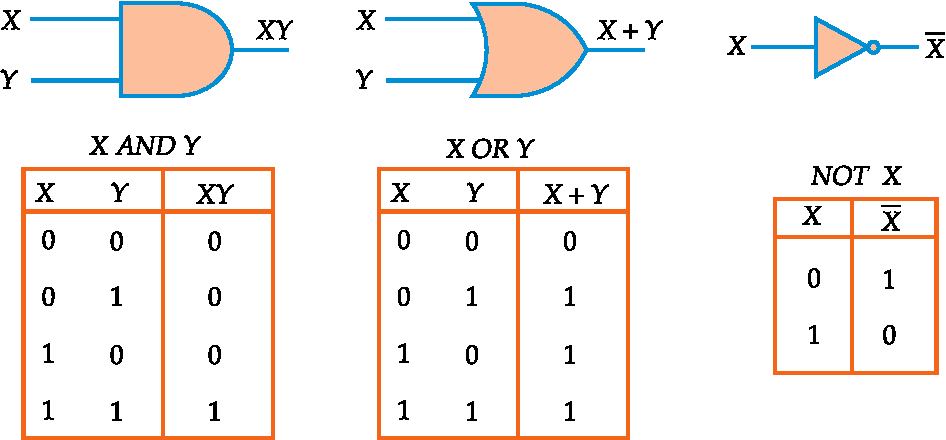
\includegraphics[height=4.5cm,width=10cm]{diagram-20211115(15)-crop}
	\caption{}
	\label{}
\end{figure}
\subsection{XOR Gate}
\begin{itemize}
	\item Another very useful gate is the exclusive OR (XOR) gate.
	\item The output of the XOR operation is true only when the values of the inputs differ.
\end{itemize}
\begin{figure}[H]
	\centering
	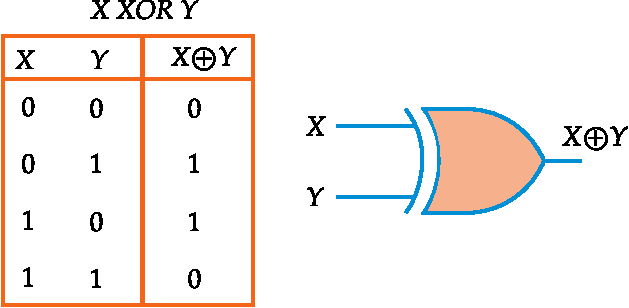
\includegraphics[height=3cm,width=6cm]{diagram-20211115(16)-crop}
	\caption{}
	\label{}
\end{figure}
\subsubsection{Equivalent Circiut of XOR Gate}
\begin{figure}[H]
	\centering
	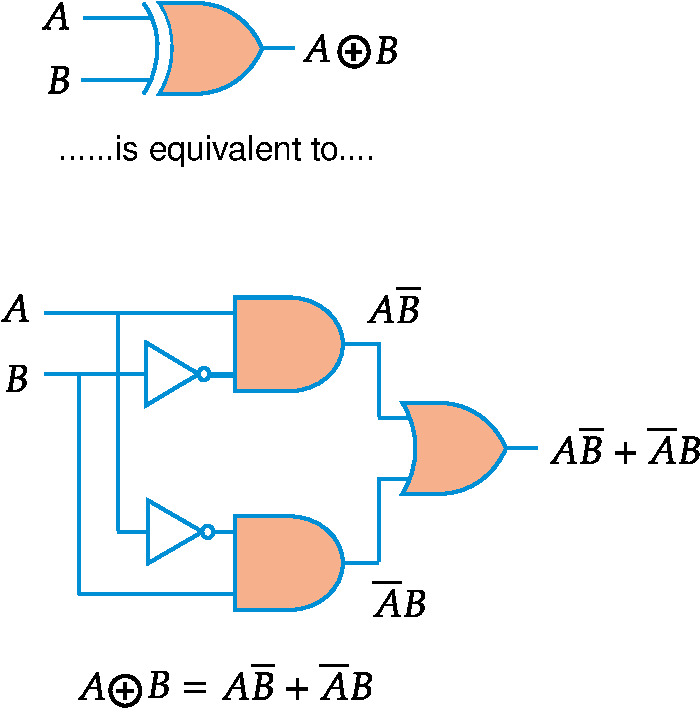
\includegraphics[height=5.2cm,width=5.5cm]{diagram-20211115(14)-crop}
	\caption{}
	\label{}
\end{figure}
\subsection{Universal gates NAND and NOR}
\begin{itemize}
	\item Two other common gates are NAND and NOR, which produce complementary output to $\mathrm{AND}$ and $\mathrm{OR}$.
\end{itemize}
\begin{figure}[H]
	\centering
	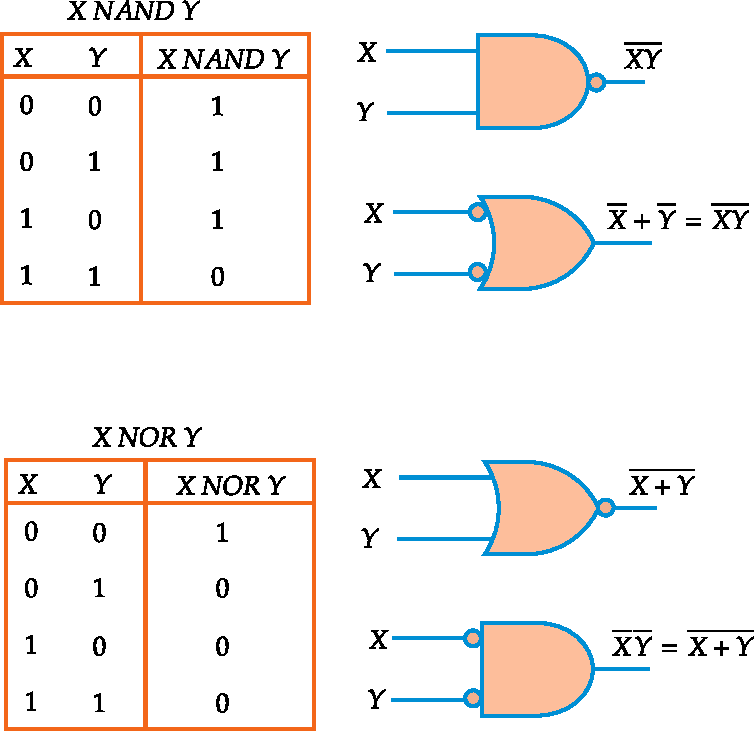
\includegraphics[height=7cm,width=7.5cm]{diagram-20211116(1)-crop}
	\caption{}
	\label{}
\end{figure}
\begin{itemize}
	\item NAND and NOR are known as universal gates because they are inexpensive to manufacture and any Boolean function can be constructed using only NAND or only NOR gates.
\end{itemize}
\subsection{Basic gates using NAND gates}
\begin{figure}[H]
	\centering
	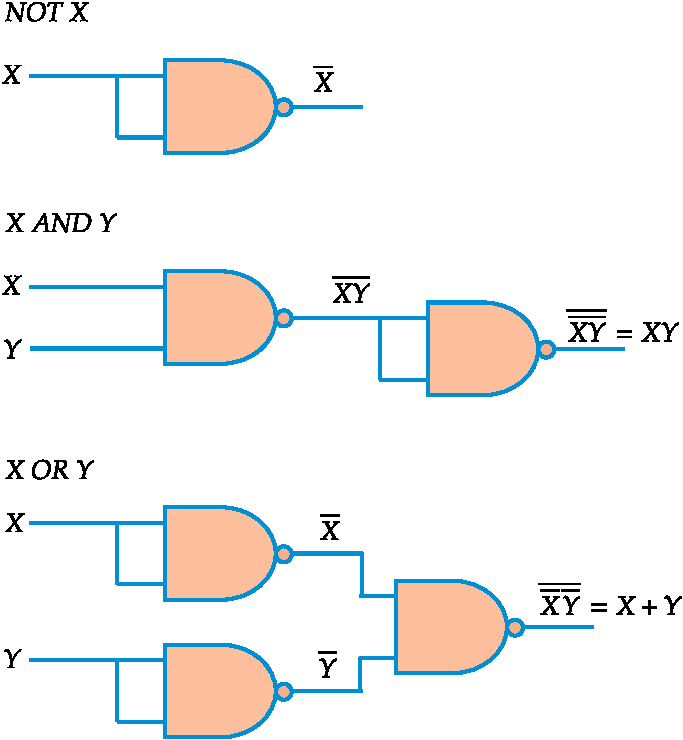
\includegraphics[height=7cm,width=6.5cm]{diagram-20211116(2)-crop}
	\caption{}
	\label{}
\end{figure}
\subsection{Basic gates using NOR gates}
\begin{figure}[H]
	\centering
	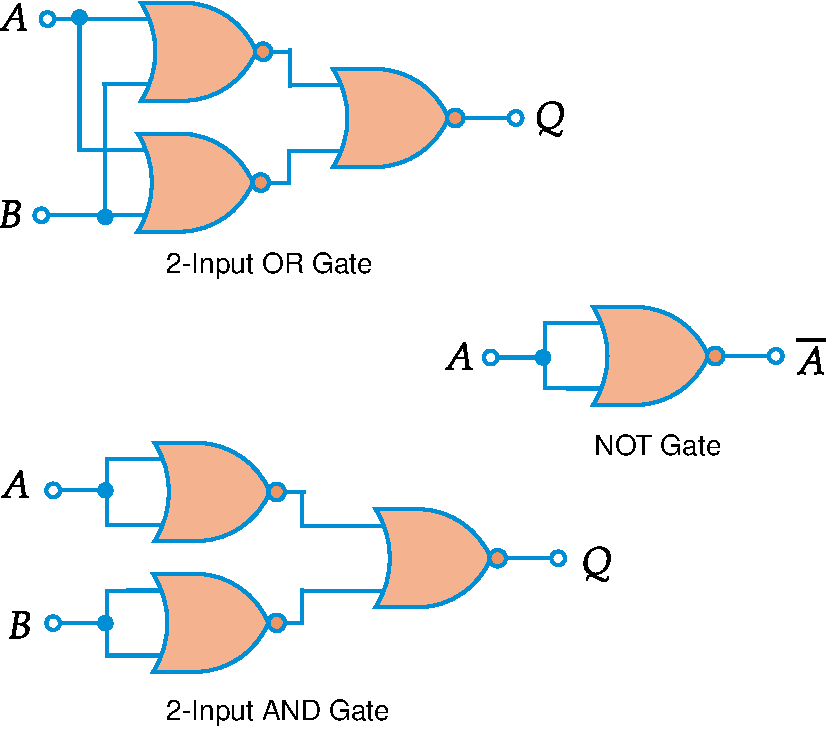
\includegraphics[height=6.3cm,width=7.5cm]{diagram-20211115(13)-crop}
	\caption{}
	\label{}
\end{figure}
\subsection{Multiple Input Gates}
\begin{figure}[H]
	\centering
	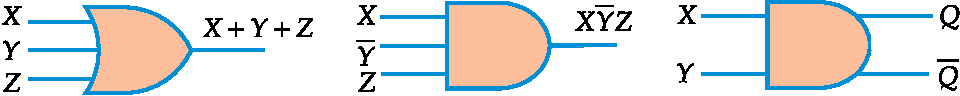
\includegraphics[height=1cm,width=10cm]{diagram-20211116(3)-crop}
	\caption{}
	\label{}
\end{figure}
\begin{exercise}
	Simplify the expression $A \bar{B} \bar{C}+\bar{A} \bar{B} \bar{C}+\bar{A} B \bar{C}+\bar{A} \bar{B} C$ and draw block diagram of the circuit using OR and AND gate
\end{exercise}
\begin{answer}
	\begin{align*}
	A \bar{B} \bar{C}+\bar{A} \bar{B} \bar{C}+\bar{A} B \bar{C}+\bar{A} \bar{B} C&=\bar{B} \bar{C}(A+\bar{A})+\bar{A} B \bar{C}+\bar{A} \bar{B} C\\&=\bar{B} \bar{C}+\bar{A} B \bar{C}+\bar{A} \bar{B} C
	\end{align*}
	\begin{figure}[H]
		\centering
		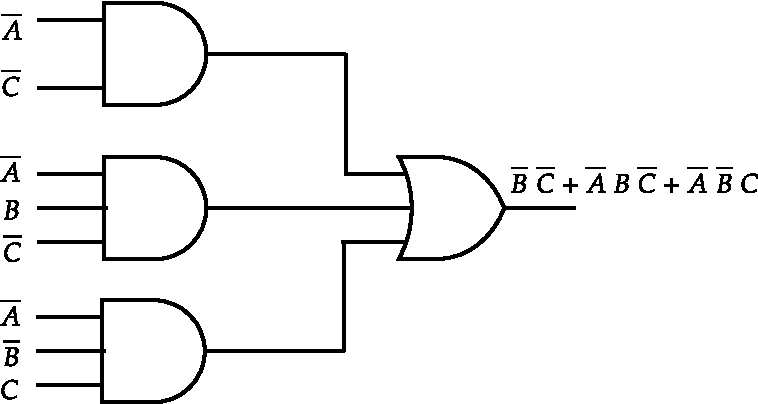
\includegraphics[height=4cm,width=8cm]{de01}
	\end{figure}
\end{answer}
\begin{exercise}
	Simplify the expression $(A+B)(B+C)(A+C)$ and draw the block diagram using OR and AND gates,
\end{exercise}
\begin{answer}
	\begin{align*}
	\intertext{The first two terms are}
	(A+B)(B+C)&=A B+A C+B B+B C\\
	&=A B+A C+B+B C\\
	&=A B+A C+B(1+C)=A B+A C+B\\
	&=B(A+1)+A C=B+A C
	\intertext{Multiply logically with the third term}
	(B+A C)(A+C)&=B A+B C+A C A+A C C\\
	&=B A+B C+A C+A C\\
	&=B A+B C+A C
	\intertext{The circuit diagram is given below}
	\end{align*}
	\begin{figure}[H]
		\centering
		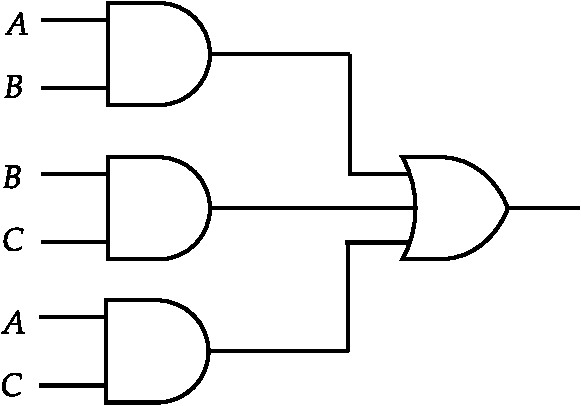
\includegraphics[height=3.2cm,width=5cm]{de02}
	\end{figure}
\end{answer}
\begin{exercise}
	Complement the following expressions\\
	\begin{tasks}(1)
		\task[\textbf{a.}]$A+B C+A B$
		\task[\textbf{b.}]$A(B+C)(\bar{C}+\bar{D})$
		\task[\textbf{c.}]$A B(\bar{C} D+\bar{B} C)$
	\end{tasks}
\end{exercise}
\begin{answer}
	\begin{align*}
	\intertext{(a)\quad complement of $A+B C+A B$ equals $\overline{A+B C+A B}$}
	\overline{A+B C+A B}&=\bar{A}(\bar{B}+\bar{C}) \overline{(A}+\bar{B})\\
	&=\overline{(A} \bar{B}+\bar{A} \bar{C}) \overline{(A}+\bar{B})\\
	&=\bar{A} \bar{B} \bar{A}+\bar{A} \bar{B} \bar{B}+\bar{A} \bar{C} \bar{A}+\bar{A} \bar{C} \bar{B}\\
	&=\bar{A} \bar{B}+\bar{A} \bar{B}+\bar{A} \bar{C}+\bar{A} \bar{C} \bar{B}\\
	&=\bar{A} \bar{B}+\bar{A} \bar{C}+\bar{A} \bar{C} \bar{B}\\
	&(\text{ since }\bar{A} \bar{B}+\bar{A} \bar{B}=\bar{A} \bar{B})\\
	&=\bar{A} \bar{B}+\bar{A} \bar{C}(1+\bar{B})=\bar{A} \bar{B}+\bar{A} \bar{C}\\
	(b) \quad \overline{A(B+C)(\bar{C}+\bar{D})}&=\bar{A}+\bar{B} \bar{C}+C D\\
	(c) \quad \quad \overline{A B(\bar{C} D+\bar{B} C)}&=\overline{A B}+\overline{\bar{C}} D+\bar{B} C
	\intertext{Boolean Algibra and Logic Gates}
	&=\bar{A}+\bar{B}+\overline{\bar{C}}+\bar{D})(\overline{\bar{B}}+\bar{C})\\
	&=\bar{A}+\bar{B}+(C+\bar{D})(B+\bar{C})
	\end{align*}
\end{answer}
\section{Logic Gates Using Transisitors}
\subsection{ 2-input Transistor OR Gate}
A simple 2-input inclusive OR gate can be constructed using RTL Resistor-transistor switches connected together as shown below with the inputs connected directly to the transistor bases. Either transistor must be saturated "ON" for an output at Q.\\
\begin{figure}[H]
	\centering
	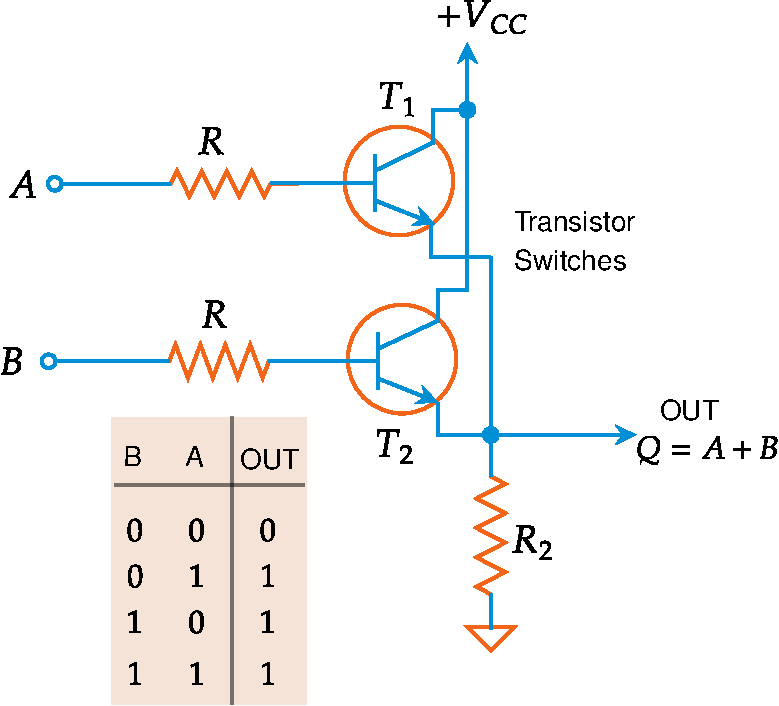
\includegraphics[height=6.2cm,width=6.9cm]{diagram-20211116(7)-crop}
\end{figure}
\subsection{ 2-input Transistor AND Gate}
A simple 2-input logic AND gate can be constructed using RTL Resistor-transistor switches connected together as shown below with the inputs connected directly to the transistor bases. Both transistors must be saturated "ON" for an output at Q.\\
\begin{figure}[H]
	\centering
	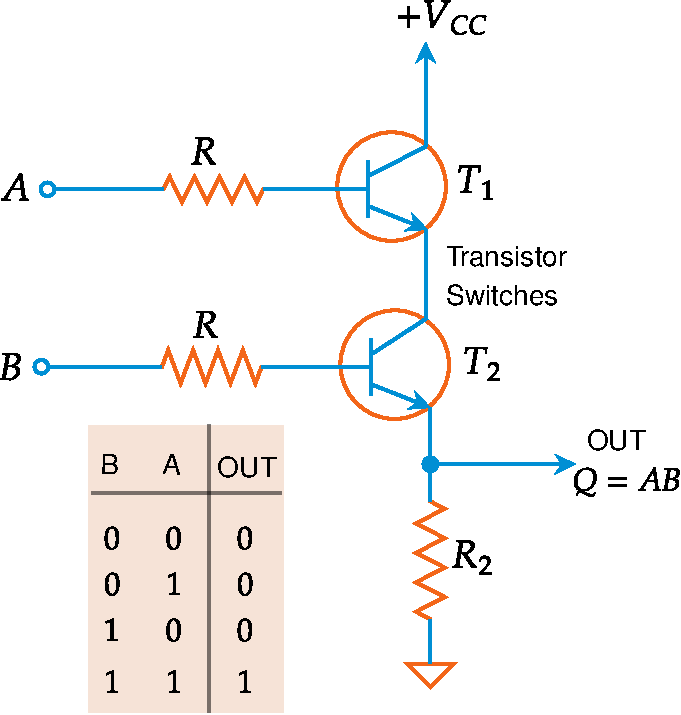
\includegraphics[height=6.2cm,width=6.2cm]{diagram-20211116(15)-crop}
	\caption{}
	\label{}
\end{figure}
\subsection{Transisitor NOT gate}
A simple 2-input logic NOT gate can be constructed using a RTL Resistor-transistor switches as shown below with the input connected directly to the transistor base. The transistor must be saturated "ON" for an inverted output "OFF" at Q.\\
\begin{figure}[H]
	\centering
	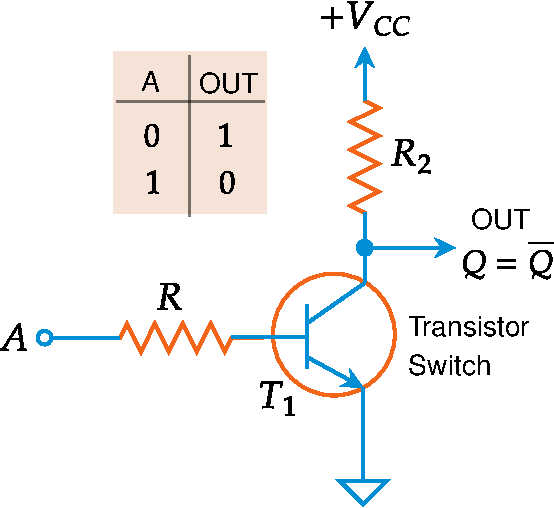
\includegraphics[height=4.5cm,width=5cm]{diagram-20211115(17)-crop}
	\caption{}
	\label{}
\end{figure}
\subsection{Transistor NAND gate}
\begin{figure}[H]
	\centering
	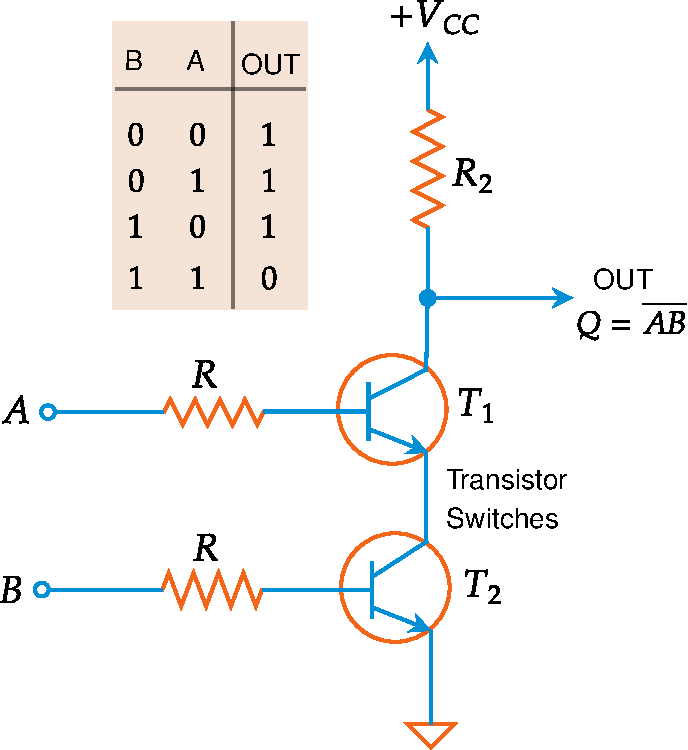
\includegraphics[height=6.1cm,width=5.5cm]{diagram-20211116-crop}
\end{figure}
\subsection{Transisitor NOR gate}
A simple 2-input logic NOR gate can be constructed using RTL Resistor-transistor switches connected together as shown below with the inputs connected directly to the transistor bases. Both transistors must be cut-off "OFF" for an output at Q.\\
\begin{figure}[H]
	\centering
	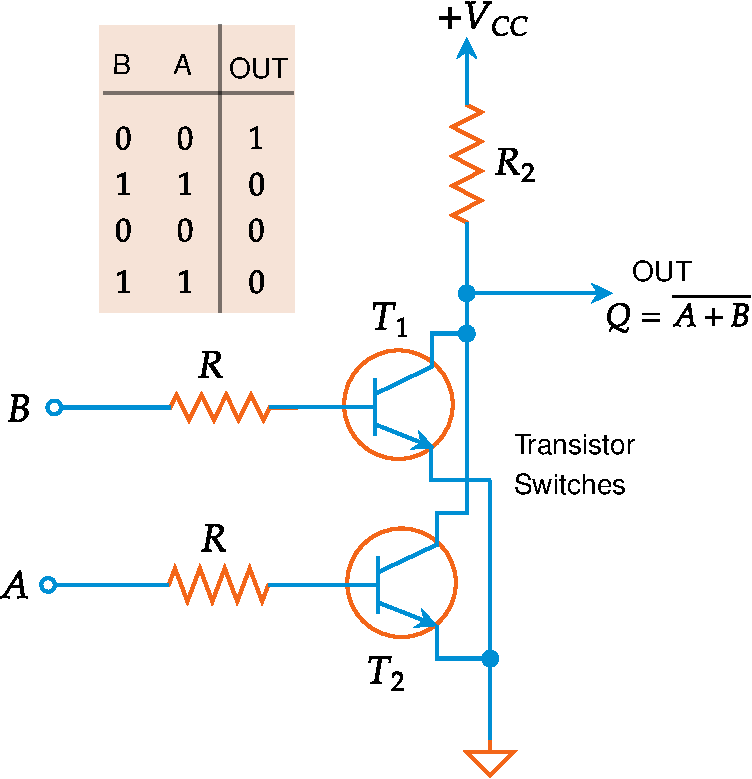
\includegraphics[height=6.3cm,width=6.1cm]{diagram-20211115(18)-crop}
	\caption{}
	\label{}
\end{figure}
\section{Simplification of Boolean expressions}
\subsection{Sum-of-Products and Product-of-Sums Boolean Expressions}
The sum-of-products expression, which is also known as minterm, contains the sum of different terms with each term being either a single literal or a product of more than one literal. It can be obtained from the truth table directly by considering those input combinations which produce logic ' 1 ' at the output. Each such input combination produces a term. The different terms are given by product of corresponding literals. The sum of all terms gives the expression.
Product-of-sums expression, which is also known as maxterm, contains the product of different terms with each term being either a single literal or a sum of more than one literal. It can be obtained from the truth table by considering those input combinations that produce logic ' 0 ' at the output. Each such input combination gives a term and product of all such terms gives the expression. Different terms are obtained by taking sum of corresponding literals. Here, ' 0 ' and ' 1 ' do mean the uncomplemented and complemented variables, respectively, unlike sum-of-products expressions where ' 0 ' and ' 1 ' do mean complemented and uncomplemented variables, respectively.
Transforming given product-of-sums expression into an equivalent sum-of-products expression is a straight forward process. Multiplying out the given expression and carrying out the obvious simplification provides the equivalent sum-of-products expression. For example,
$$
\begin{aligned}
(A+B) \cdot(\bar{A}+\bar{B}) &=A \cdot \bar{A}+A \cdot \bar{B}+B \cdot \bar{A}+B \cdot \bar{B} \\
&=0+A \cdot \bar{B}+B \cdot \bar{A}+0=A \cdot \bar{B}+\bar{A} \cdot B
\end{aligned}
$$
A given sum-of-products expression can be transformed into an equivalent product-of-sums expression by (a) taking dual of given expression (b) multiplying out different terms to get the sum-of-products form (c) removing redundancy and (d) taking a dual to get the equivalent product-of-sums expression. \\Let us consider the example, $A \cdot B+\bar{A} \cdot \bar{B}$ :
$$
\begin{aligned}
\text{Dual of given expression }&=(A+B) \cdot(\bar{A}+\bar{B})\\
(A+B) \cdot(\bar{A}+\bar{B}) &=A \cdot \bar{A}+A \cdot \bar{B}+B \cdot \bar{A}+B \cdot \bar{B} \\
&=0+A \cdot \bar{B}+B \cdot \bar{A}+0\\&=A \cdot \bar{B}+\bar{A} \cdot B\\
\text{Dual of } (A \cdot \bar{B}+\bar{A} \cdot B)&=(A+\bar{B}) \cdot(\bar{A}+B)\\
\text{Therefore, } A \cdot B+\bar{A} \cdot \bar{B}&=(A+\bar{B}) \cdot(\bar{A}+B)
\end{aligned}
$$

\subsection{Karnaugh Map Method}
Karnaugh map (K-map) is a graphical representation of
the logic system. It can be drawn directly from either
minterm (sum-of-products) or maxterm (product-of-
sums) Boolean expressions. Drawing a Karnaugh map
from truth table involves an additional step of writing
the minterm or maxterm expression depending upon
whether it is desired to have minimized sum-of-products
or a minimized product-of-sums expression.
\subsection{Construction of Karnaugh Map}
An $n$-variable Karnaugh map has $2^{n}$ squares and each possible input is allotted a square. In case of a minterm Karnaugh map, ' 1 ' is placed in all those squares for which the output is ' 1 ' and ' 0 ' is placed in all those squares for which the output is ' 0 '. For simplicity, 0's are omitted. An $X$ is placed in squares corresponding to 'don't care' conditions. In the case of a maxterm Karnaugh map, a ' 1 ' is placed in all those squares for which the output is ' 0 ' and a ' 0 ' is placed for input entries corresponding to a ' 1 ' output. Again 0's are omitted for simplicity and an $X$ is placed in squares corresponding to 'don't care' conditions.\\
The process of construction of 2,3 and 4 variable Karnaugh maps is illustrated in the following examples.\\
The choice of terms identifying different rows and columns of a Karnaugh map is not unique for a given number of variables. The only condition to be satisfied is that the designation of adjacent rows and adjacent columns should be the same except for one of the literals being complemented. Also, the extreme rows and extreme columns are considered adjacent. Some of the possible designation styles for two-, three- and four-variable minterm Karnaugh maps are given in Figs. \ref{2-variable K map}, \ref{3-variable K map} and \ref{4-variable K map}, respectively.\\
\begin{minipage}{0.45\textwidth}
	\begin{figure}[H]
		\centering
		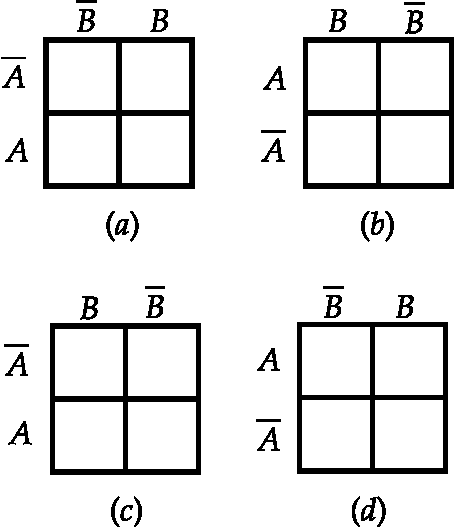
\includegraphics[height=4cm,width=4cm]{DE-10}
		\caption{Two-variable Karnaugh map.}
		\label{2-variable K map}
	\end{figure}
\end{minipage}
\begin{minipage}{0.45\textwidth}
	\begin{figure}[H]
		\centering
		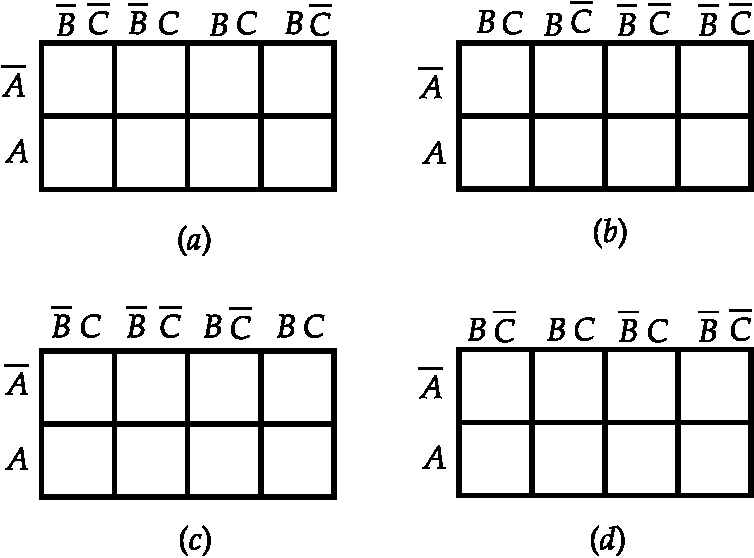
\includegraphics[height=5cm,width=6.5cm]{DE-11}
		\caption{Three-Variable Karnaugh map}
		\label{3-variable K map}
	\end{figure}
\end{minipage}
\begin{figure}[H]
	\centering
	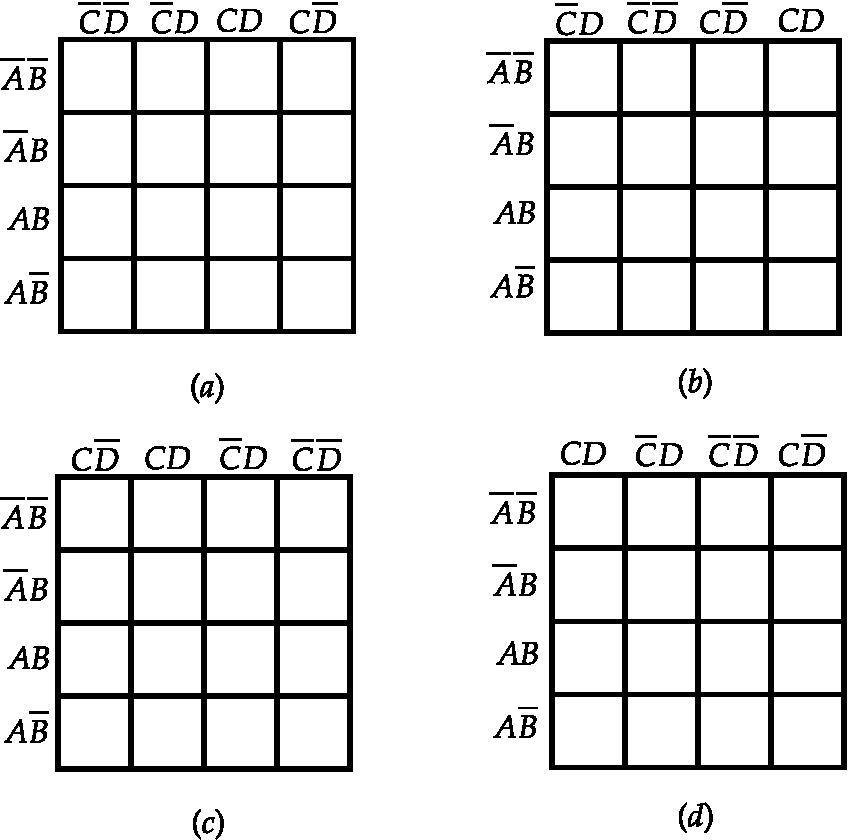
\includegraphics[height=7cm,width=7.5cm]{DE-12}
	\caption{Four-Variable Karnaugh map}
	\label{4-variable K map}
\end{figure}
However not necessary to account for all optional entries. Only those optional combinations that can be used to advantage should be used.\\
Having made groups with all 1's having been accounted for, the minimum 'sum-of-products' or the 'product-of-sums' expressions can be written directly from Karnaugh map. Figures \ref{2-variable K map sop},\ref{3-variable K map sop} and \ref{4-variable K map sop} illustrate the construction of minterm and maxterm Karnaugh maps for two-, three- and four-variable Boolean expressions, respectively.
\begin{figure}[H]
	\centering
	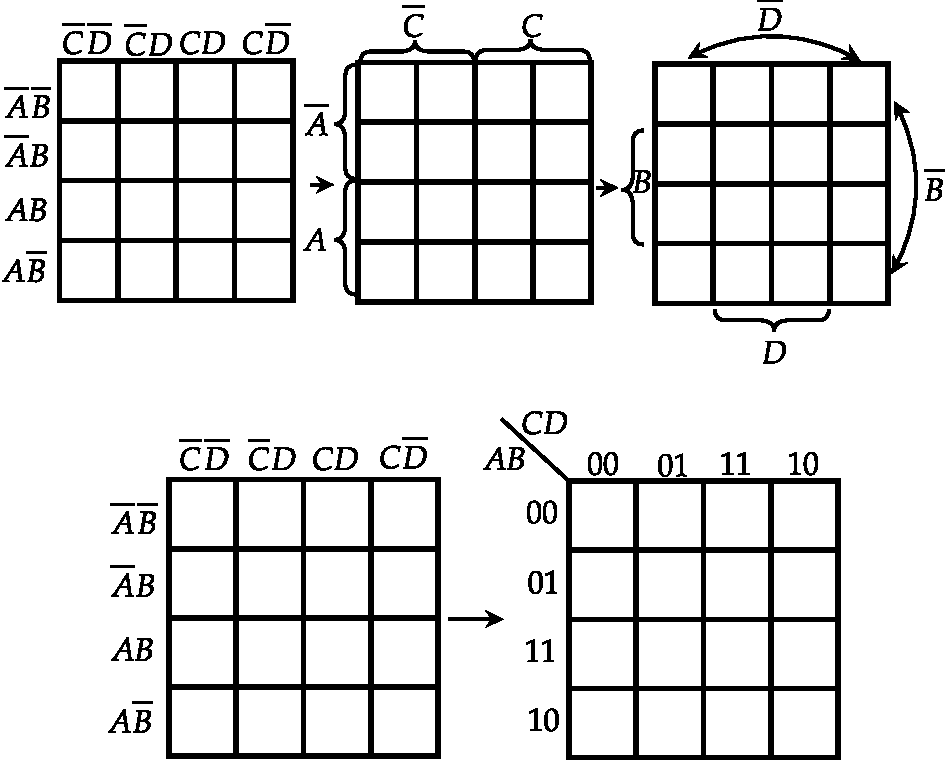
\includegraphics[height=7cm,width=9cm]{DE-13}
	\caption{Different styles of row and columns identification.}
	\label{}
\end{figure}
\begin{figure}[H]
	\centering
	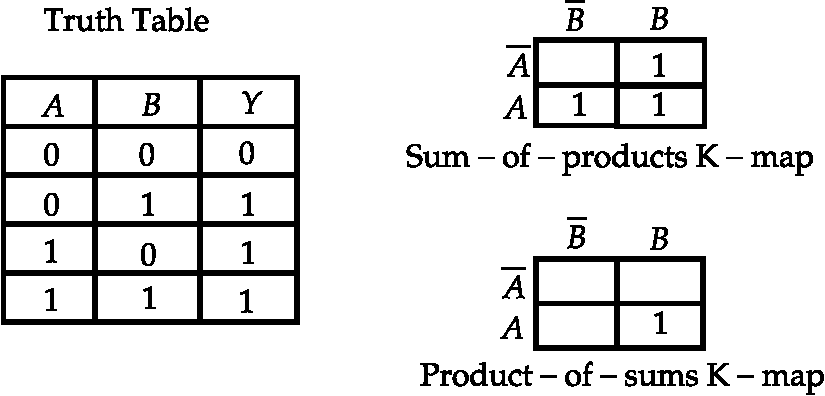
\includegraphics[height=3.7cm,width=7.5cm]{DE-14}
	\caption{Two-variable-Karnaugh maps.}
	\label{2-variable K map sop}
\end{figure}
\begin{figure}[H]
	\centering
	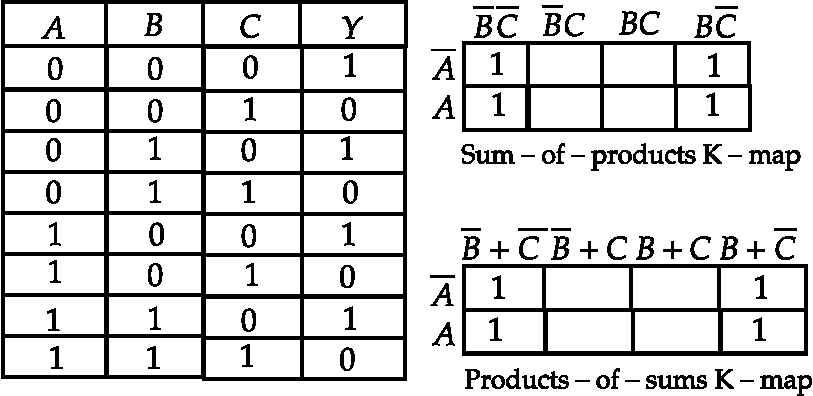
\includegraphics[height=4.2cm,width=9cm]{DE-15}
	\caption{Three-variable-Karnaugh maps.}
	\label{3-variable K map sop}
\end{figure}
\begin{figure}[H]
	\centering
	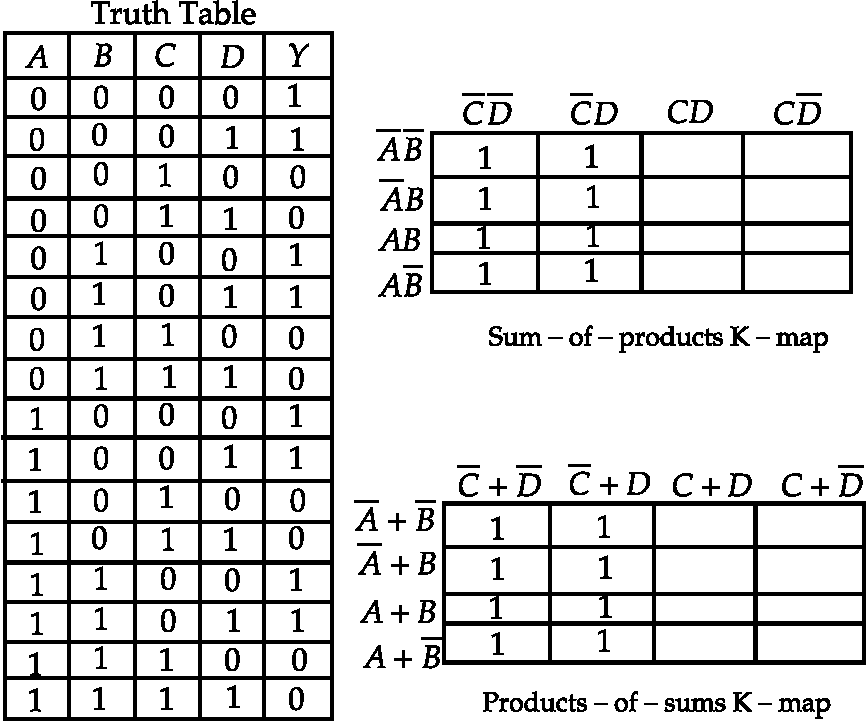
\includegraphics[height=8cm,width=9cm]{DE-16}
	\caption{Four Variable-Karnaugh maps.}
	\label{4-variable K map sop}
\end{figure}

\section{Multiplexer(MUX)}
Multiplex means many into one. A multiplexer is a circuit with many inputs but only one output. By applying control signals, we can steer any input to the output. Thus it is also called a data selector and control inputs are termed select inputs. A MUX is represented by many input and single output line.The internal structure of MUX is a rotatory switch.
\\ It is used for parellel to series conversion. It's also called as universal combinational circuit.

\begin{figure}[H]
	\centering
	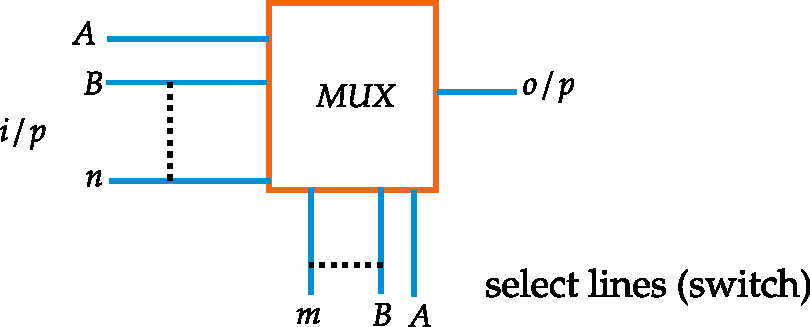
\includegraphics[height=3cm,width=7cm]{EDE-40}
	\caption{}
	\label{}
\end{figure}
If the number of input lines in a MUX is $N$, then,
\begin{align*}
N&=2^n\\
\text{Where, } n&=\text{number of select lines.}
\end{align*}
\subsection{$2 \times 1$ MUX}
Here, the number of input lines,N
\begin{align*}
N&=2^{n}=2\\
\text{Then,number of select lines } n&=1
\end{align*}
\begin{example}
 For a two level AND-OR circuit can be equally represented by
	\begin{tasks}(2)
		\task[\textbf{a.}]AND-AND
		\task[\textbf{b.}]OR-AND
		\task[\textbf{c.}]NOR-NOR
		\task[\textbf{d.}] NAND-NAND
	\end{tasks}

		\begin{figure}[H]
			\centering
			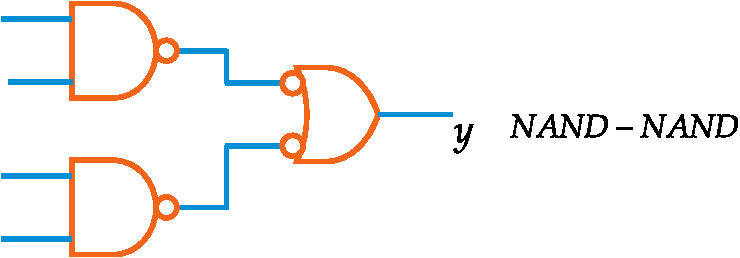
\includegraphics[height=2.4cm,width=7cm]{EDE-42}
		\end{figure}
	
\end{example}
\subsection{4$\times$ 1 MUX}
\begin{figure}[H]
	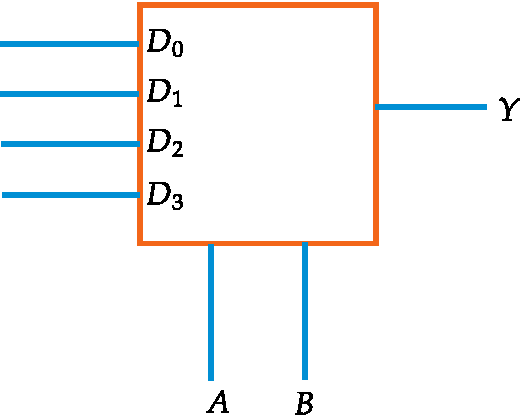
\includegraphics[height=3.5cm,width=4.5cm]{DE-01}
\end{figure}
\text{Output }\quad y=$\bar{A}\bar{B}D_0+\bar{A}BD_1+A\bar{B}D_2+ABD_3$
\subsection{8$\times 1$ MUX}
\begin{align*}
	2^n&=8\\
 \text{ number of select lines, }n&=3\\
	y&=\bar{A}\bar{B} \bar{C}D_0+\bar{A}\bar{B} CD_1+
	\bar{A}B\bar{C}D_2+\bar{A}BCD_3+
	A \bar{B}\bar{C}D_4+A\bar{B}CD_5+
	AB\bar{C}D_5+ABCD_7
\end{align*}
\section
{Minimization of logical expression of using MUX:}
1.\quad  Minimize
\begin{figure}[H]
	\centering
	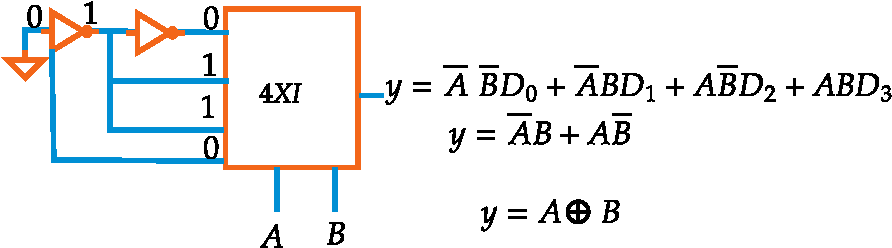
\includegraphics[height=2.7cm,width=9cm]{EDE-43}
\end{figure}
2.\quad  Minimize
\begin{figure}[H]
	\centering
	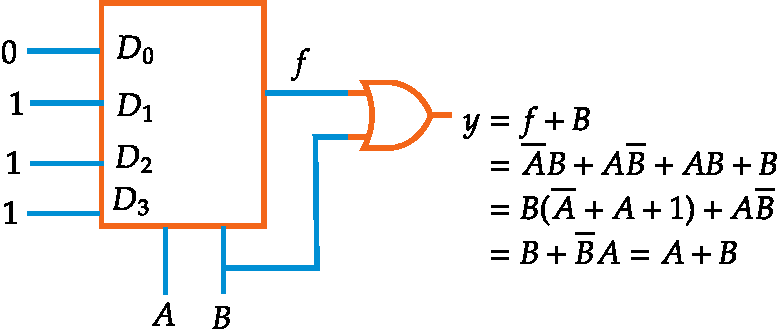
\includegraphics[height=3.2cm,width=8.5cm]{EDE-44}
\end{figure}
\subsection{Implementation of higher order MUX by using $2\times 1$MUX:}
\begin{enumerate}
	\item $4\times1$ MUX by $2\times 1$ MUX
	\begin{figure}[H]
		\centering
		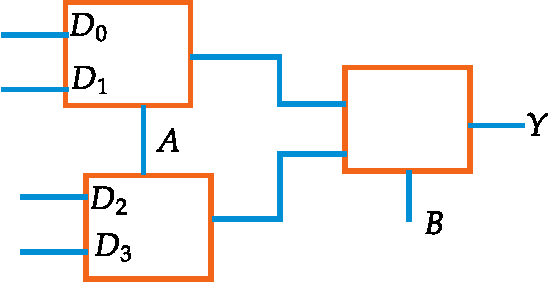
\includegraphics[height=3cm,width=5cm]{EDE-45}
	\end{figure}
	\begin{align*}
	\text{Alternate method to find the number of MUX}\\
	\begin{tabular}{p{0.5cm}|p{0.5cm}}
	2&4\\\hline
	2&2\\\hline
	&1
	\end{tabular}\\
	2+ 1=3\\
	\text{ three, } 2 \times 1\text{ MUX } \text{is required}
	\end{align*}
 $16\times 1$ MUX by $2\times 1$ MUX
	\begin{align*}
	\begin{array}{c|c}
	2 & 16 \\
	\hline 2 & 8\\
\hline	2 & 4 \\
	\hline 2 & 2 \\
	\hline & 1
	\end{array}=8+4+2+1\Rightarrow 15, (\text{Fifteen,}\quad 2 \times 1\text{ MUX
		Required.})
	\end{align*}
	similarly,
	\item $256 \times 1$ MUX by $16 \times 1$ MUX
	\begin{align*}
	\begin{tabular}{c|c}
	16 & 256 \\
	\hline 16 & 16\\
	\hline  &1
	\end{tabular}\quad 16+1=17 (\text{Seventeen, }16 \times 1 \text{MUX is required}) .
	\end{align*}
\end{enumerate}
\subsubsection{Implementation of Logic gates by using $2 \times 1$ MUX and $u \times 1$ MUX:}
1.\quad NOT gate:
\begin{figure}[H]
	\centering
	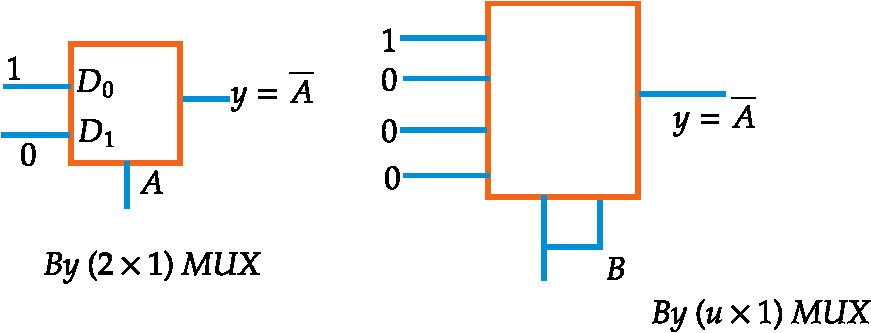
\includegraphics[height=2.8cm,width=4.5cm]{EDE-46}
\end{figure}
\renewcommand*{\arraystretch}{1.5}
$\begin{array}{|c|c|c|}
\hline\text { Logic gate } & \text { 2$\times$1 MUX } & \text { 4$\times$1 MUX } \\
\hline \text { NOT } & 1 & 1 \\
\hline \text { AND } & 1 & 1 \\
\hline \text { OR } & 1 & 1 \\
\hline \text { NAND } & 2 & 1\\
\hline \text { NOR } & 2 & 1\\
\hline \text { EX-OR } & 2 & 1\\
\hline \text { EX-NOR } & 2 & 1\\	\hline
\end{array}$\\\\\\
2. \quad For the implementation of AND gate and XOR gate the number of 2X1 MUX required.
\begin{tasks}(4)
	\task[\textbf{a.}] 1,1
	\task[\textbf{b.}]1,2
	\task[\textbf{c.}]2,1
	\task[\textbf{d.}] 2,2
\end{tasks}
\begin{answer}
	\begin{align*}
	\text { I MUX for AND, 2MUX for XOR }
	\end{align*}
	So the correct answer is \textbf{Option (b)}
\end{answer}
\subsubsection{Demultiplexer:}
A de MUX performs the reverse operation of MUX.
\begin{figure}[H]
	\centering
	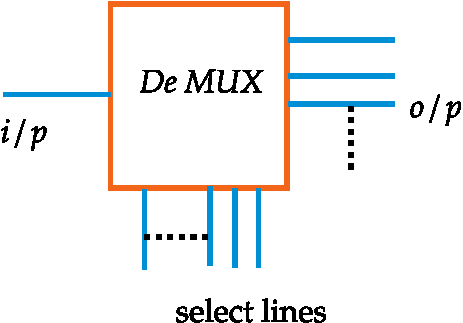
\includegraphics[height=3.3cm,width=4.7cm]{EDE-47}
\end{figure}
\begin{itemize}
	\item Number of outputs $=2^{n}$ where $n \rightarrow$ select lines
	\item  De MUX is also called as data detector.
	\item By setting the input to true (1), the demux behaves as decoder.
\end{itemize}
\subsubsection{$1 \times 4$ DEMUX}
\begin{figure}[H]
	\centering
	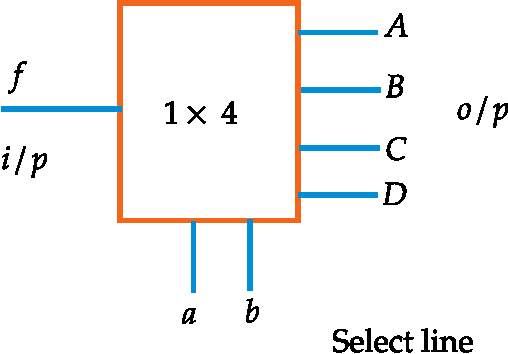
\includegraphics[height=3.5cm,width=5.1cm]{EDE-48}
\end{figure}
\section{Flip-Flop}
\subsubsection{Sequential Circuit}
Digital output are required to be generated in accordance with sequence in which input signals are received, which is not possible with the combinational circuit generated should depend on present and past history of input. Such circuit is called as sequential circuit.\\\\
	\subsubsection{SR-Latch:}
	\begin{figure}[H]
		\centering
		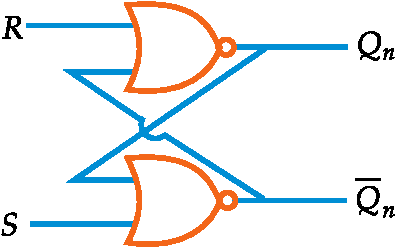
\includegraphics[height=2.8cm,width=4.5cm]{EDE-01}
	\end{figure}
\subsubsection{Truth Table:}
\begin{tabular}{|c|c|c|c|}
	\hline$C L K$ & $R$ & $S$ & $Q_{n+1}$ \\
	\hline 1 & 0 & 0 & $Q_{n}$ \\
	\hline 1 & 0 & 1 & 1 \\
	\hline 1 & 1 & 0 & 0 \\
	\hline 1 & 1 & 1 & Invalid \\
	\hline 0 & $X$ & $X$ & $Q_{n}$ \\
	\hline
\end{tabular}
$\mathrm{X}$ : Input either 0 or 1
\subsubsection{ S-R Flip Flop with NAND Gate: }
\begin{figure}[H]
	\centering
	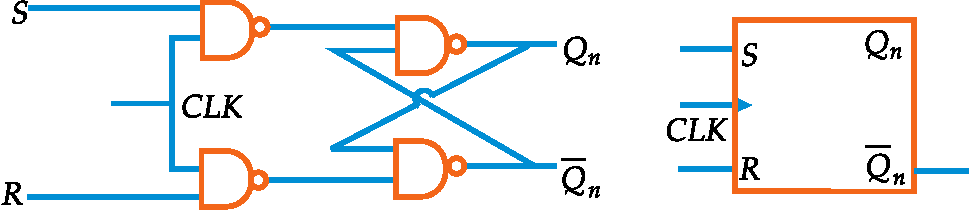
\includegraphics[height=2.1cm,width=11cm]{EDE-02}
\end{figure}
\subsubsection{D-Flip Flop (Delay): }
When $\mathrm{S}=\mathrm{D}, \bar{R}=D$, Now SR becomes $\mathrm{D}$ type Flip Flop.
\begin{figure}[H]
	\centering
	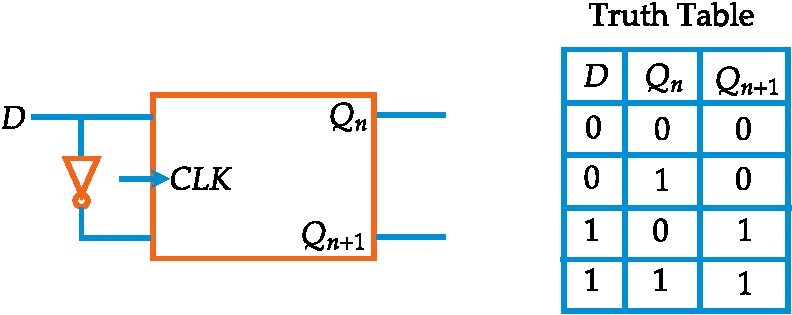
\includegraphics[height=3.2cm,width=7.7cm]{EDE-03}
\end{figure}
\subsubsection{ J-K Flip Flop: }
$S=J\left(\bar{Q}_{n}\right) ; R=K\left(Q_{n}\right)$
\begin{figure}[H]
	\centering
	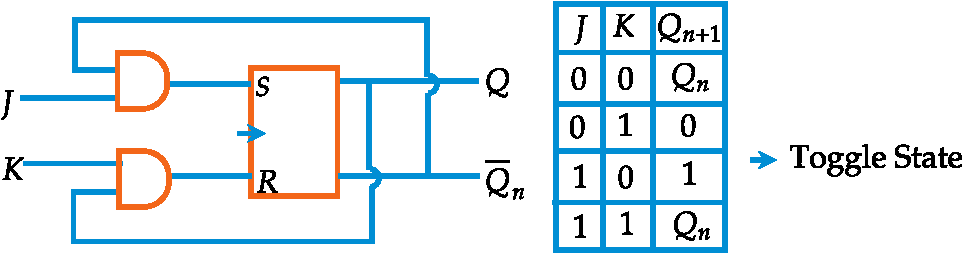
\includegraphics[height=2.4cm,width=9.5cm]{EDE-04}
\end{figure}
\begin{note}
Problem in JK flip flop is race around condition.
\end{note}
\subsubsection{T-type (Toggle) Flip Flop:} $\mathrm{J}=\mathrm{K}=\mathrm{T}$ then $\mathrm{T}=$ Flip Flop.
 \begin{figure}[H]
 	\centering
 	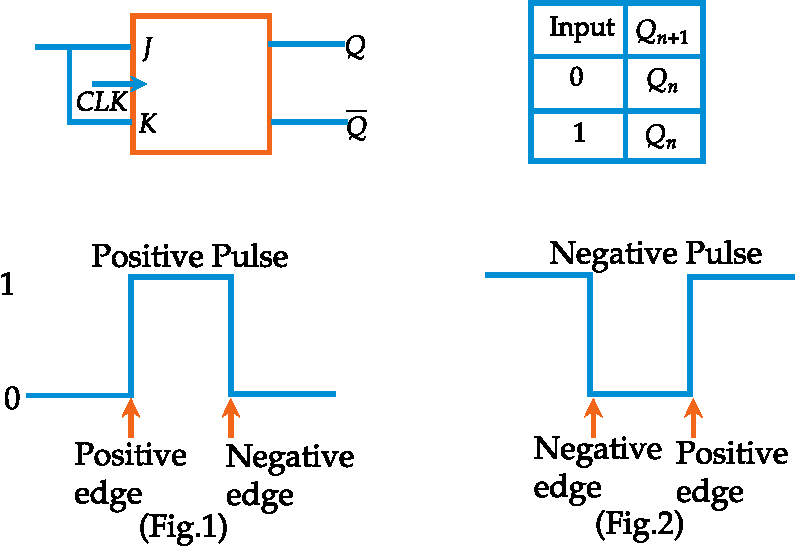
\includegraphics[height=5.4cm,width=7.5cm]{EDE-05}
 \end{figure}
 A clock pulse may be either positive or negative. A positive clock source remains at 0 during the interval between pulses and goes 0 to 1 during the occurrence of a pulse. The pulse goes through two signal transitions; from 0 to 1 and return from 1 to 0, positive transition is defined as the positive edge and the negative transition as the negative edge.\\
\subsubsection{Time Diagram Representation:}
 \begin{figure}[H]
 	\centering
 	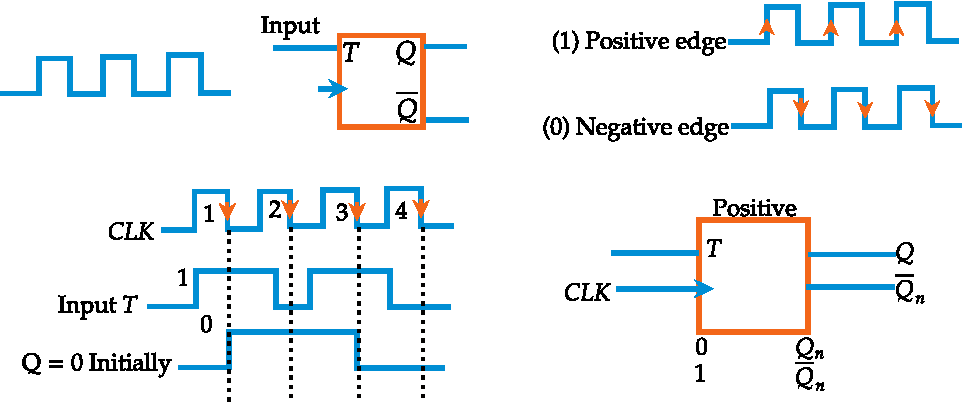
\includegraphics[height=4.8cm,width=10.5cm]{EDE-06}
 \end{figure}
\subsubsection{If we take positive edge:}
 \begin{figure}[H]
 	\centering
 	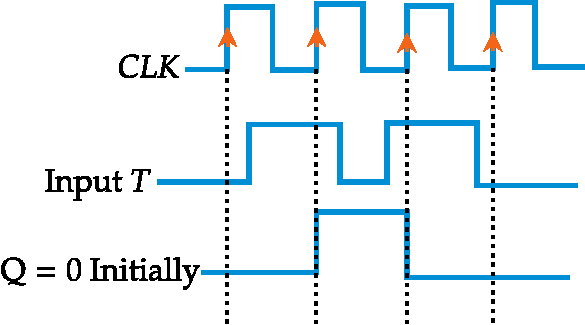
\includegraphics[height=3cm,width=5.4cm]{EDE-07}
 \end{figure}
 	\section{Counters}
 	\begin{enumerate}
 		\item Asynchronous or ripple or serial 
 		\item Synchronous or parallel or fast
 		\item (i) Ring counter (ii) Twisted tail or thomson or mobious (Type of shift registers)
 	\end{enumerate}
 \begin{enumerate}
 	\item \textbf{Asychronous Counter:} No, common clock-clock is output of previous flip-flop.
 	\item In synchronous counter common clock is used.
 \end{enumerate}
\begin{enumerate}
\item  	What is meaning of MOD-12 counter $\Rightarrow$ number of states are 12 .\\
1. $0-11 \rightarrow 12$ states\qquad
2. $2-13 \rightarrow 12$ states\\
3. $3-14 \rightarrow 12$ states\qquad
4. $1-12 \rightarrow 12$ states\\
 	MOD 12 means divide by 12 .
 	\begin{figure}[H]
 		\centering
 		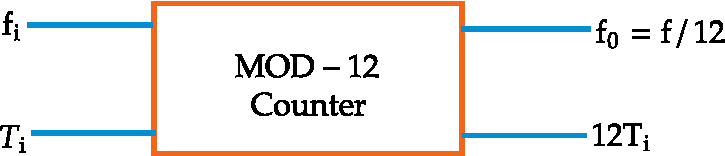
\includegraphics[height=1.3cm,width=6cm]{EDE-13}
 	\end{figure}
 \subsubsection{ Asynchronous Counter: }
 		\begin{figure}[H]
 		\centering
 		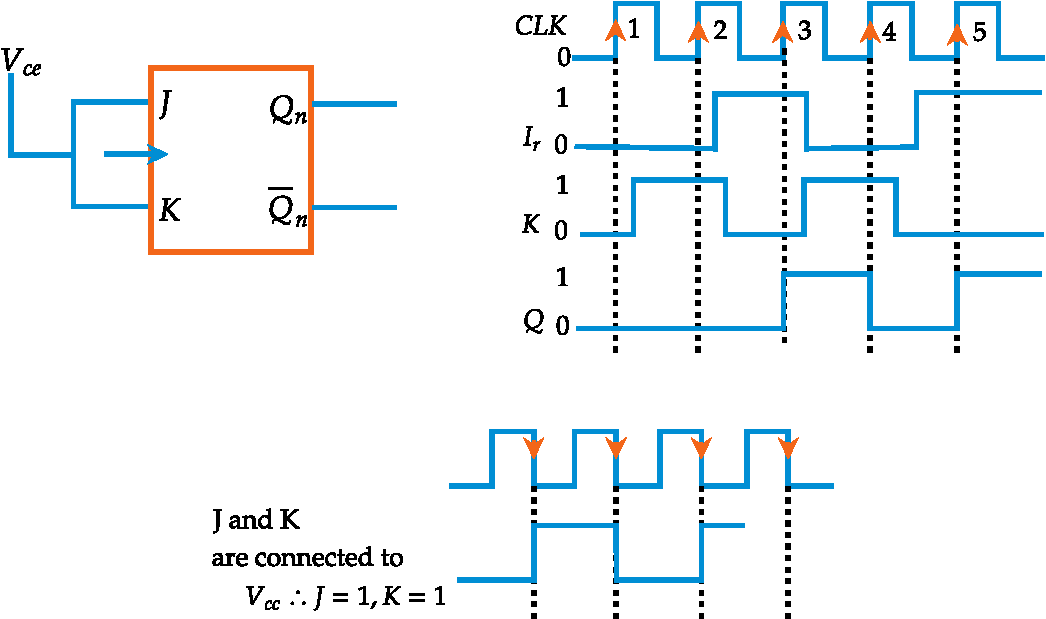
\includegraphics[height=6cm,width=10cm]{EDE-14}
 	\end{figure}
 \begin{note}
 		1. Total number of flip-flop required for Mod-N counter $\mathrm{N}=2^{n}$.\\
 	2. 3 bit means MOD-8 counter $\Rightarrow$ MOD $8=2^{3}$ means 3 Flip-Flop required.\\
 	3. 4 bit $\rightarrow 16 \mathrm{MOD} \rightarrow 2^{4} \rightarrow 4$ Flip Flop required
 \end{note}
 \subsubsection{ MOD-8 Asychronous Counter: }
 	\begin{figure}[H]
 		\centering
 		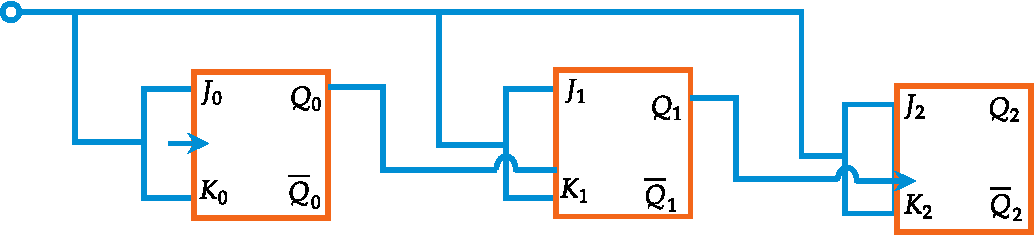
\includegraphics[height=2.3cm,width=9cm]{EDE-15}
 	\end{figure}
 \begin{figure}[H]
 	\centering
 	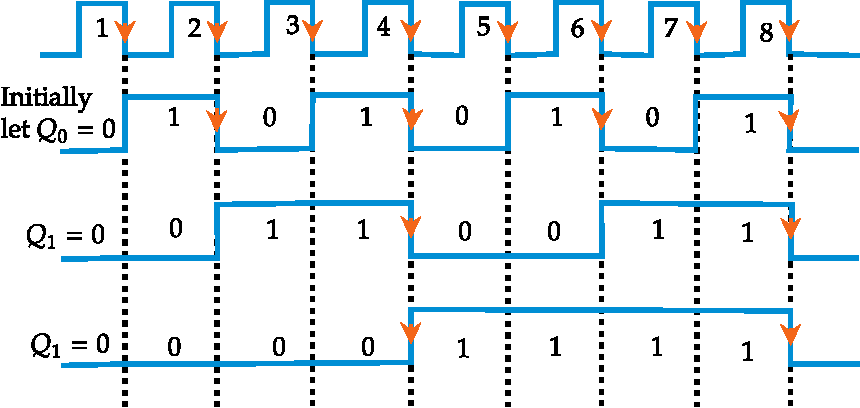
\includegraphics[height=5cm,width=10cm]{EDE-16}
 \end{figure}
\begin{align*}
	&\text { Truth Tuble }\\
	&\begin{array}{|c|c|c|c|}
		\hline C L K & Q_{2} & Q_{1} & Q_{0} \\
		\hline 1 & 0 & 0 & 0 \\
		\hline 2 & 0 & 0 & 1 \\
		\hline 3 & 0 & 1 & 0 \\
		\hline 4 & 0 & 1 & 1 \\
		\hline 5 & 1 & 0 & 0 \\
		\hline 6 & 1 & 0 & 1 \\
		\hline 7 & 1 & 1 & 0 \\
		\hline 8 & 1 & 1 & 1 \\
		\hline
	\end{array}
\end{align*}
 	Edge $\rightarrow$ Positive $\rightarrow$ (i) up counter (ii) Down counter \\
 	Edge $\rightarrow$ Negative $\rightarrow$ (i) up counter (ii) Down counter
 	\begin{figure}[H]
 		\centering
 		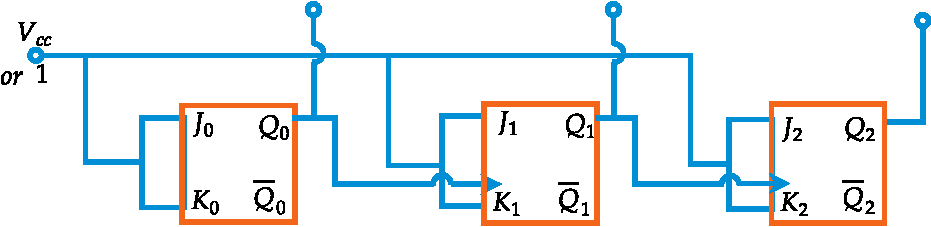
\includegraphics[height=2.5cm,width=9.5cm]{EDE-17}
 	\end{figure}
 	$\mathrm{Q}_{2}, \mathrm{Q}_{1}, \mathrm{Q}_{0}$ are standard output\\
 	\textbf{Case (i):} If the output is of first flip-flop is given as circuit to next flip-flop it will act as up counter.\\
 	\textbf{Case (ii):} If $\bar{Q}$ of 1 st flip flop is given as circuit to next flip-flop it will act as down counter.
 	\begin{figure}[H]
 	\centering
 	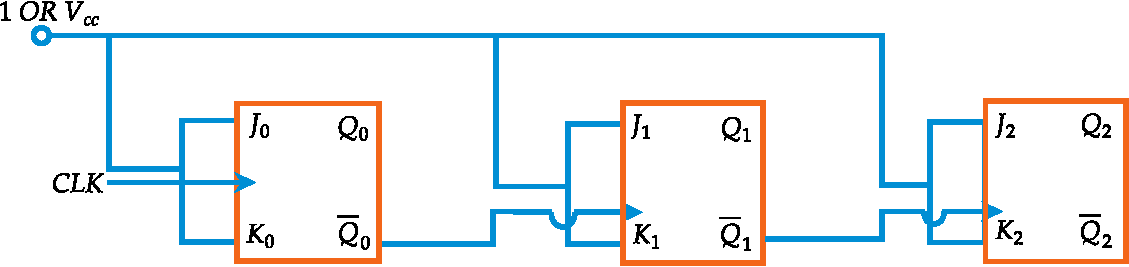
\includegraphics[height=2.6cm,width=9.8cm]{	EDE-18}
 \end{figure}
\subsubsection{Synchronous Counter}
(i) Common clock is there (ii) There are fast \\
Widely used if MOD is in form of 2N then design is simple. If MOD is not in form of 2N then design by use of K-map.\\
	Example: MOD-10 UP counter.
	\begin{figure}[H]
		\centering
		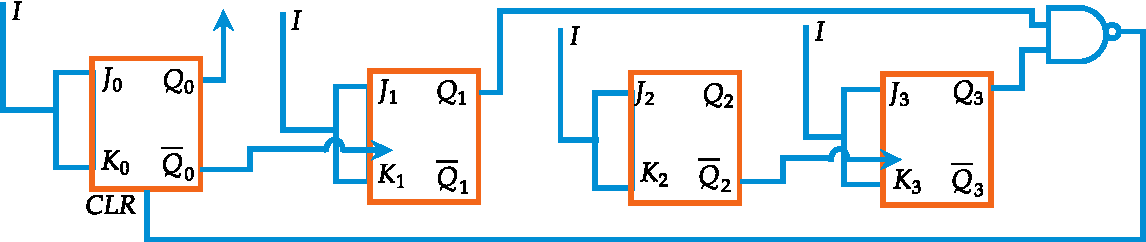
\includegraphics[height=2.5cm,width=12cm]{EDE-21}
	\end{figure}
\begin{figure}[H]
	\centering
	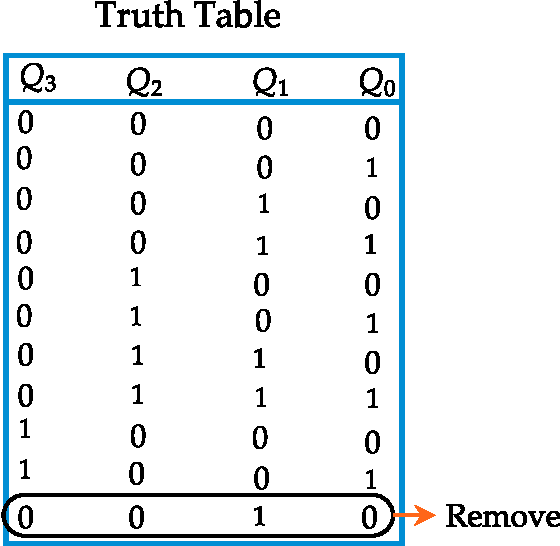
\includegraphics[height=5cm,width=4.5cm]{EDE-22}
\end{figure}
\subsubsection{Shift Register}
Register's are group of flip-flop.\\
To store $n$-bits $n$-bits $n$-flip-flop are required in register. \\
Depending upon input and output registers can be classified as\\
(1) SISO [Serial input serial output]\quad
(3) PISO [Parallel in serial output]\\
(2) SIPO [Serial input parallel out]\quad
(4) PIPO [Parallel input parallel output]\\
\subsubsection{ 4-Bit SISO}
\begin{figure}[H]
	\centering
	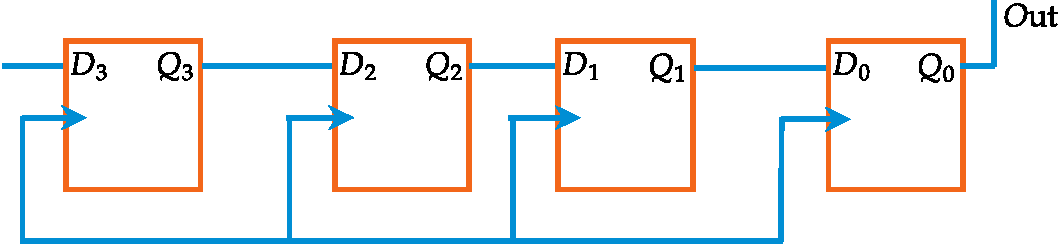
\includegraphics[height=2.4cm,width=10cm]{EDE-27}
\end{figure}
To provide $n$-bit data in $(n-1)$-clk pulse required, \\
To store $n$-bit data $n$-click pulse required.\\
S\subsubsection{IPO(4-Bit)}
\begin{figure}[H]
	\centering
	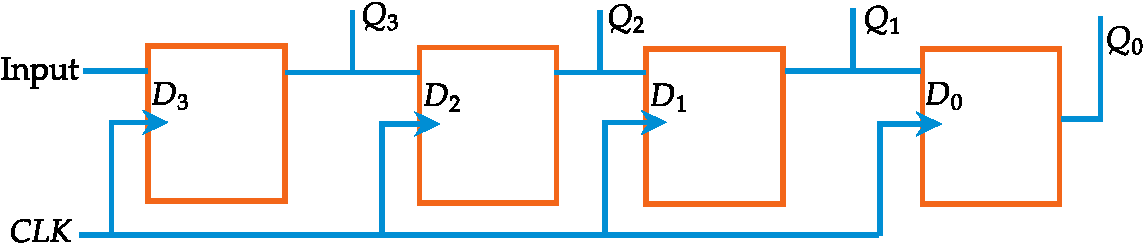
\includegraphics[height=2.2cm,width=10cm]{EDE-28}
\end{figure}
To provide $n$-bit data in $n$-clk pulse required, to provide parallel out no circuit pulse required.\\
\subsubsection{ PISO }
\begin{figure}[H]
	\centering
	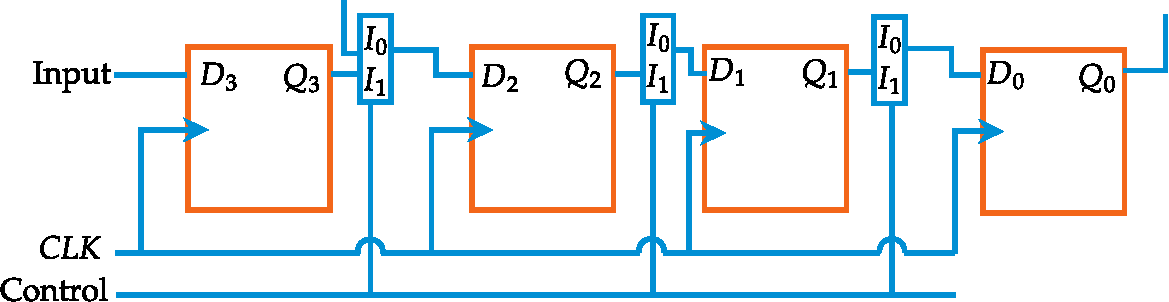
\includegraphics[height=2.6cm,width=10cm]{EDE-29}
\end{figure}
Control $0 \rightarrow$ Parallel input, Control $1 \rightarrow$ Serial output\\
\subsubsection{ PIPO}
\begin{figure}[H]
	\centering
	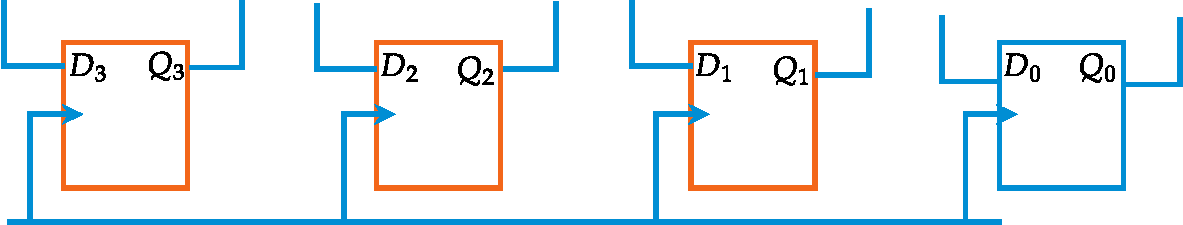
\includegraphics[height=2cm,width=10cm]{EDE-30}
\end{figure}
 Initial contents of 4-bit SIPO, ring shift register, shown in figure is 0110 . After 3 clock pulses are applied, what are contents of shift register.
\begin{figure}[H]
	\centering
	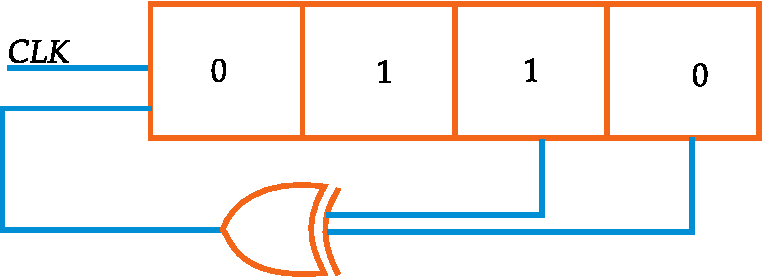
\includegraphics[height=2.4cm,width=6cm]{EDE-31}
\end{figure}
\begin{answer}
	After 1 st clock $\rightarrow 1011,2$ nd clock $\rightarrow 0101$, 3rd clock $\rightarrow 1010$. So content are 1010 .
\end{answer}
\subsubsection{Ring Counter:}
Design MOD-5 ring counter. After each 10 steps is reads again 0000.
\begin{figure}[H]
	\centering
	\includegraphics[height=2.6cm,width=11cm]{EDE-34}
\end{figure}
Ring counter is shift register with feedback applied last flip-flop output $Q$ to input of first flip flop.\\
Ring counter is one bit is logic one and it will rotate with clock.\\
In $n$-bit ring counter number of use state is $n$.\\
Number of unused states in $n$-bit ring counter is $2^{n}-n$.
\begin{figure}[H]
	\centering
	\includegraphics[height=5.7cm,width=8cm]{EDE-39}
\end{figure}
\textbf{Johnson Counter } or (Twisted Ring Counter) or Switch Tail Counter or Creeping Counter or Mobies Counter or Walking Counter.
\begin{figure}[H]
	\centering
	\includegraphics[height=2.4cm,width=9.5cm]{EDE-35}
\end{figure}
\subsubsection{ Equivalent Circuit: }
\begin{figure}[H]
	\centering
	\includegraphics[height=2.4cm,width=7cm]{EDE-36}
\end{figure}
\subsubsection{ Truth Table : }
\begin{figure}[H]
	\centering
	\includegraphics[height=5cm,width=5cm]{EDE-37}
\end{figure}
In Johnson counter with $n$-flip-flop maximum possible states are $2 n$ states or maximum uses states. Unused states are $2^{n}-2 n$.\\
$50 \%$ duty cycle.\\
When a Johnson counter is working in uses state the operation frequency $f / 2 n$.\\
 \end{enumerate}










\newpage
\begin{abox}
	Practice set-1
\end{abox}
\begin{enumerate}
	\item A signal of frequency $10 k H z$ is being digitalized by an A/D converter. A possible sampling time which can be used is
	{	\exyear{NET/JRF(JUNE-2011)}}
	\begin{tasks}(4)
		\task[\textbf{A.}] $100 \mu s$
		\task[\textbf{B.}] $40 \mu s$
		\task[\textbf{C.}] $60 \mu \mathrm{s}$
		\task[\textbf{D.}] $200 \mu s$
	\end{tasks}
	\item Consider the digital circuit shown below in which the input $C$ is always high (1).\\
	\begin{figure}[H]
		\centering
		\includegraphics[height=3cm,width=7cm]{diagram-20211018-crop}
	\end{figure}
	The truth table for the circuit can be written as
	\begin{align*}
	\renewcommand*{\arraystretch}{1.2}
	\begin{tabular}{|p{1.5cm}|p{1.5cm}|p{1.5cm}|}
	\hline $\mathrm{A}$ & $\mathrm{B}$ & $\mathrm{Z}$ \\
	\hline 0 & 0 & 1 \\
	\hline 0 & 1 & 0 \\
	\hline 1 & 0 & 1 \\
	\hline 1 & 1 & 1 \\
	\hline
	\end{tabular}
	\end{align*}
	The entries in the $Z$ column (vertically) are
	{	\exyear{NET/JRF(JUNE-2011)}}
	\begin{tasks}(4)
		\task[\textbf{A.}]  1010
		\task[\textbf{B.}] 0100
		\task[\textbf{C.}] 1111
		\task[\textbf{D.}] 1011
	\end{tasks}
	\item A counter consists of four flip-flops connected as shown in the figure:\\
	\begin{figure}[H]
		\centering
		\includegraphics[height=3.5cm,width=7.5cm]{diagram-20211018(3)-crop}
	\end{figure}
	If the counter is initialized as $A_{0} A_{1} A_{2} A_{3}=0110$, the state after the next clock pulse is
	{\exyear{NET/JRF(DEC-2011)}}
	\begin{tasks}(4)
		\task[\textbf{A.}] 1000
		\task[\textbf{B.}]  0001
		\task[\textbf{C.}] 0011
		\task[\textbf{D.}] 1100
	\end{tasks}
	\item The output, $\mathrm{O}$, of the given circuit in cases I and II, where\\
	\textbf{Case I:}\quad $\mathrm{A}, \mathrm{B}=1 ; \mathrm{C}, \mathrm{D}=0 ; \mathrm{E}, \mathrm{F}=1$ and $\mathrm{G}=0$\\
	\textbf{Case II:}\quad $\mathrm{A}, \mathrm{B}=0 ; \mathrm{C}, \mathrm{D}=0: \mathrm{E}, \mathrm{F}=0$ and $\mathrm{G}=1$ are respectively.
	{\exyear{NET/JRF(JUNE-2012)}}
		\begin{tasks}(4)
			\task[\textbf{A.}] 1,0
			\task[\textbf{B.}] 0,1
			\task[\textbf{C.}] 0,0
			\task[\textbf{D.}] 1,1
		\end{tasks}
	\begin{minipage}{0.45\textwidth}
		\begin{figure}[H]
			\centering
			\includegraphics[height=4cm,width=5.5cm]{e-11}
		\end{figure}
	\end{minipage}
	\item  The logic circuit shown in the figure below Implements the Boolean expression
	{\exyear{NET/JRF(DEC-2012)}}
	\begin{figure}[H]
		\centering
		\includegraphics[height=2.5cm,width=6cm]{e-14}
	\end{figure}
	\begin{tasks}(4)
		\task[\textbf{A.}] $y=\overline{A \cdot B}$
		\task[\textbf{B.}] $y=\bar{A} \cdot \bar{B}$
		\task[\textbf{C.}] $y=A \cdot B$
		\task[\textbf{D.}] $y=A+B$
	\end{tasks}
	\item If the analog input to an 8 -bit successive approximation ADC is increased from $1.0 \mathrm{~V}$ to $2.0 \mathrm{~V}$, then the conversion time will
	{\exyear{NET/JRF(JUNE-2013)}}
	\begin{tasks}(2)
		\task[\textbf{A.}] Remain unchanged
		\task[\textbf{B.}] Double
		\task[\textbf{C.}] Decrease to half its original value
		\task[\textbf{D.}] Increase four times
	\end{tasks}
	\item If one of the inputs of a J-K flip flop is high and the other is low, then the outputs $Q$ and $\bar{Q}$
	{	\exyear{NET/JRF(DEC-2013)}}
	\begin{tasks}(1)
		\task[\textbf{A.}] Oscillate between low and high in race around condition
		\task[\textbf{B.}] Toggle and the circuit acts like a $T$ flip flop
		\task[\textbf{C.}] Are opposite to the inputs
		\task[\textbf{D.}] Follow the inputs and the circuit acts like an $R-S$ flip flop
	\end{tasks}
	\item A 4 -variable switching function is given by $f=\sum(5,7,8,10,13,15)+d(0,1,2)$, where $d$ is the do-not-care-condition. The minimized form of $f$ in sum of products (SOP) form is
	{\exyear{NET/JRF(DEC-2013)}}
	\begin{tasks}(4)
		\task[\textbf{A.}] $\bar{A} \bar{C}+\overline{B D}$
		\task[\textbf{B.}] $A \bar{B}+C \bar{D}$
		\task[\textbf{C.}]  $A D+B C$
		\task[\textbf{D.}] $\overline{B D}+B D$
	\end{tasks}
	\item For the logic circuit shown in the below\\
	\begin{figure}[H]
		\centering
		\includegraphics[height=3.5cm,width=7cm]{e-29}
	\end{figure}
	A simplified equivalent circuit is
	{	\exyear{NET/JRF(JUNE-2014)}}
	\begin{tasks}(2)
		\task[\textbf{A.}] 
		\begin{figure}[H]
			\centering
			\includegraphics[height=1cm,width=3.3cm]{e-29a}
		\end{figure}
		\task[\textbf{B.}] \begin{figure}[H]
			\centering
			\includegraphics[height=2cm,width=4.5cm]{e-29b}
		\end{figure}
		\task[\textbf{C.}] \begin{figure}[H]
			\centering
			\includegraphics[height=2cm,width=4.5cm]{e-29c}
		\end{figure}
		\task[\textbf{D.}] \begin{figure}[H]
			\centering
			\includegraphics[height=2cm,width=4.5cm]{e-29d}
		\end{figure}
	\end{tasks}
	\item The state diagram corresponding to the following circuit is
	{	\exyear{NET/JRF(DEC-2015)}}
	\begin{figure}[H]
		\centering
		\includegraphics[height=3cm,width=6.5cm]{e41}
	\end{figure}
	\begin{tasks}(2)
		\task[\textbf{A.}] \begin{figure}[H]
			\centering
			\includegraphics[height=2cm,width=3.8cm]{e41a}
		\end{figure}
		\task[\textbf{B.}] \begin{figure}[H]
			\centering
			\includegraphics[height=2cm,width=3.8cm]{e41b}
		\end{figure}
		\task[\textbf{C.}] \begin{figure}[H]
			\centering
			\includegraphics[height=2cm,width=3.8cm]{e41c}
		\end{figure}
		\task[\textbf{D.}] \begin{figure}[H]
			\centering
			\includegraphics[height=2cm,width=3.8cm]{e41d}
		\end{figure}
	\end{tasks}
	\item In the schematic figure given below, assume that the propagation delay of each logic gate is $t_{\text {gate }}$.\\
	\begin{figure}[H]
		\centering
		\includegraphics[height=2.5cm,width=5cm]{e44}
	\end{figure}
	The propagation delay of the circuit will be maximum when the logic inputs $A$ and $B$ make the transition
	{\exyear{NET/JRF(JUNE-2016)}}
	\begin{tasks}(2)
		\task[\textbf{A.}] $(0,1) \rightarrow(1,1)$
		\task[\textbf{B.}] $(1,1) \rightarrow(0,1)$
		\task[\textbf{C.}] $(0,0) \rightarrow(1,1)$
		\task[\textbf{D.}] 	$(0,0) \rightarrow(0,1)$
	\end{tasks}
	\item Which of the following circuits implements the Boolean function
	$$F(A, B, C)=\sum(1,2,4,6) ?$$
	{	\exyear{NET/JRF(DEC-2016)}}
	\begin{tasks}(2)
		\task[\textbf{A.}] \begin{figure}[H]
			\centering
			\includegraphics[height=3.3cm,width=4.5cm]{e47a}
		\end{figure}
		\task[\textbf{B.}] \begin{figure}[H]
			\centering
			\includegraphics[height=3.3cm,width=4.5cm]{e47b}
		\end{figure}
		\task[\textbf{C.}] \begin{figure}[H]
			\centering
			\includegraphics[height=3.3cm,width=4.5cm]{e47c}
		\end{figure}
		\task[\textbf{D.}] \begin{figure}[H]
			\centering
			\includegraphics[height=3.3cm,width=4.5cm]{e47d}
		\end{figure}
	\end{tasks}
	\item A $2 \times 4$ decoder with an enable input can function as a
	{	\exyear{NET/JRF(JUNE-2017)}}
	\begin{tasks}(2)
		\task[\textbf{A.}] $4 \times 1$ multiplexer
		\task[\textbf{B.}] $1 \times 4$ demultiplexer
		\task[\textbf{C.}] $4 \times 2$ encoder
		\task[\textbf{D.}] $4 \times 2$ priority encoder
	\end{tasks}
	\item In the figures below, $X$ and $Y$ are one bit inputs. The circuit which corresponds to a one bit comparator is
	{	\exyear{NET/JRF(JUNE-2017)}}
	\begin{tasks}(2)
		\task[\textbf{A.}] \begin{figure}[H]
			\centering
			\includegraphics[height=2.8cm,width=5.5cm]{e58a}
		\end{figure}
		\task[\textbf{B.}] \begin{figure}[H]
			\centering
			\includegraphics[height=2.8cm,width=5.5cm]{e58b}
		\end{figure}
		\task[\textbf{C.}] \begin{figure}[H]
			\centering
			\includegraphics[height=2.8cm,width=5.5cm]{e58c}
		\end{figure}
		\task[\textbf{D.}] \begin{figure}[H]
			\centering
			\includegraphics[height=2.8cm,width=5.5cm]{e58d}
		\end{figure}
	\end{tasks}
	\item The circuit below comprises of $D$-flip flops. The output is taken from $Q_{3}, Q_{2}, Q_{1}$ and $Q_{0}$ as shown in the figure.\\
	\begin{figure}[H]
		\centering
		\includegraphics[height=3.6cm,width=9cm]{e66}
	\end{figure}
	the binary number given by the string $Q_{3}, Q_{2}, Q_{1} Q_{0}$ changes for every clock pulse that is applied to the CLK input. If the output is initialized at 0000 , the the corresponding sequence of decimal numbers that repeats itself, is
	{	\exyear{NET/JRF(DEC-2017)}}
	\begin{tasks}(2)
		\task[\textbf{A.}] $3,2,1,0$
		\task[\textbf{B.}] $1,3,7,14,12,8$
		\task[\textbf{C.}] $1,3,7,15,12,14,0$
		\task[\textbf{D.}] $1,3,7,15,14,12,8,0$
	\end{tasks}
	\item In the following $J K$ flip-flop circuit, $J$ and $K$ inputs are tied together to $+V_{C C} .$ If the input is a clock signal of frequency $f$, the frequency of the output $Q$ is
	{	\exyear{NET/JRF(JUNE-2018)}}
	\begin{figure}[H]
		\centering
		\includegraphics[height=3cm,width=6cm]{e69}
	\end{figure}
	\begin{tasks}(4)
		\task[\textbf{A.}] $f$
		\task[\textbf{B.}] $2 f$
		\task[\textbf{C.}] $4 f$,
		\task[\textbf{D.}] $\frac{f}{2}$
	\end{tasks}
	\item Which of the following gates can be used as a parity checker?
	{	\exyear{NET/JRF(JUNE-2018)}}
	\begin{tasks}(2)
		\task[\textbf{A.}] An OR gate
		\task[\textbf{B.}] A NOR gate
		\task[\textbf{C.}] An exclusive OR (XOR) gate
		\task[\textbf{D.}] An AND gate
	\end{tasks}
	\item The full scale of a 3 -bit digital-to-analog (DAC) converter is $7 V$. Which of the following tables represents the output voltage of this 3 -bit DAC for the given set of input bits?
	{	\exyear{NET/JRF(JUNE-2018)}}
	\begin{tasks}(2)
		\task[\textbf{A.}] 
		\begin{align*}
		\begin{tabular}{|p{2cm} |p{2.5cm}|}
		\hline
		Input bits& Output voltage\\\hline
		000&0\\	\hline
		001&1\\	\hline
		010&2\\	\hline
		011&3\\	\hline
		\end{tabular}
		\end{align*}
		\task[\textbf{B.}] 	\begin{align*}
		\begin{tabular}{|p{2cm} |p{2.5cm}|}
		\hline
		Input bits& Output voltage\\\hline
		000&0\\	\hline
		001&1.25\\	\hline
		010&2.5\\	\hline
		011&3.75\\	\hline
		\end{tabular}
		\end{align*}
		\task[\textbf{C.}] 	\begin{align*}
		\begin{tabular}{|p{2cm} |p{2.5cm}|}
		\hline
		Input bits& Output voltage\\\hline
		000&1.25\\	\hline
		001&2.5\\	\hline
		010&3.75\\	\hline
		011&5\\	\hline
		\end{tabular}
		\end{align*}
		\task[\textbf{D.}] 	\begin{align*}
		\begin{tabular}{|p{2cm} |p{2.5cm}|}
		\hline
		Input bits& Output voltage\\\hline
		000&1\\	\hline
		001&2\\	\hline
		010&3\\	\hline
		011&4\\	\hline
		\end{tabular}
		\end{align*}
	\end{tasks}
	\item Consider the following circuit, consisting of an RS flip-flop and two AND gates.\\
	\begin{figure}[H]
		\centering
		\includegraphics[height=2cm,width=7cm]{e74}
	\end{figure}
	Which of the following connections will allow the entire circuit to act as a $JK$  flip-flop?
	{\exyear{NET/JRF(DEC-2018)}}
	\begin{tasks}(1)
		\task[\textbf{A.}]  Connect $Q$ to pin 1 and $\bar{Q}$ to pin 2
		\task[\textbf{B.}] Connect $Q$ to pin 2 and $\bar{Q}$ to pin 1
		\task[\textbf{C.}] Connect $Q$ to $K$ input and $\bar{Q}$ to $J$ input
		\task[\textbf{D.}] Connect $Q$ to $J$ input and $\bar{Q}$ to $K$ input
	\end{tasks}
	\item The truth table below gives the value $Y ( A , B , C)$  where $A , B$ and $C$ are binary variables.
	The output Y can be represented by
	{\exyear{NET/JRF(DEC-2018)}}
	\begin{tasks}(1)
		\task[\textbf{A.}] $Y=\overline{A B} C+\bar{A} B \bar{C}+A \bar{B} C+A B \bar{C}$
		\task[\textbf{B.}] $Y=\bar{A} \bar{B} \bar{C}+\bar{A} B C+A \bar{B} \bar{C}+A B C$
		\task[\textbf{C.}] $Y=\overline{A B C}+\bar{A} B C+A \overline{B C}+A B C$
		\task[\textbf{D.}] $Y=\bar{A} \bar{B} \bar{C}+\bar{A} B \bar{C}+A \overline{B C}+A B \bar{C}$
	\end{tasks}
	\begin{align*}
	\renewcommand*{\arraystretch}{1.2}
	\begin{tabular}{|p{1cm}|p{1cm}|p{1cm}|p{1cm}|}
	\hline$A$ & $B$ & $C$ & $Y$ \\
	\hline 0 & 0 & 0 & 1 \\
	\hline 0 & 0 & 1 & 0 \\
	\hline 0 & 1 & 0 & 0 \\
	\hline 0 & 1 & 1 & 1 \\
	\hline 1 & 0 & 0 & 1 \\
	\hline 1 & 1 & 0 & 0 \\
	\hline 1 & 1 & 1 & 1 \\
	\hline
	\end{tabular}
	\end{align*}
	\item Let Y denote the output in the following logical Circuit.\\
	\begin{figure}[H]
		\centering	\includegraphics[height=3.5cm,width=5cm]{diagram-20211029(5)-crop}
	\end{figure}
	If $Y=A B+\overline{C D}$, the gates $G_{1}$ and $G_{2}$ must, respectively, be
	{\exyear{NET/JRF(JUNE-2019)}}
	\begin{tasks}(2)
		\task[\textbf{A.}] OR and NAND
		\task[\textbf{B.}] NOR and OR
		\task[\textbf{C.}] AND and NAND
		\task[\textbf{D.}] NAND and OR
	\end{tasks}
	\item In the 3 -bit register shown below, $Q_{1}$ and $Q_{3}$ are the least and the most significant bits of the output, respectively.\\
	\begin{figure}[H]
		\centering
		\includegraphics[height=3.5cm,width=8cm]{diagram-20211029(13)-crop}
	\end{figure}
	If $Q_{1}, Q_{2}$ and $Q_{3}$ are set to zero initially, then the output after the arrival of the second falling clock (CLK) edge is
	{\exyear{NET/JRF(JUNE-2020)}}
	\begin{tasks}(4)
		\task[\textbf{A.}]  001
		\task[\textbf{B.}] 100
		\task[\textbf{C.}]  011
		\task[\textbf{D.}]  110
	\end{tasks}
	\item The Boolean equation $Y=\bar{A} B C+\bar{A} B \bar{C}+A \bar{B} \bar{C}+A \bar{B} C$ is to be implemented using only twoinput NAND gates. The minimum number of gates required is
	{\exyear{NET/JRF(JUNE-2020)}}
	\begin{tasks}(4)
		\task[\textbf{A.}] 3
		\task[\textbf{B.}] 4
		\task[\textbf{C.}] 5
		\task[\textbf{D.}] 6
	\end{tasks}
\end{enumerate}
 \colorlet{ocre1}{ocre!70!}
\colorlet{ocrel}{ocre!30!}
\setlength\arrayrulewidth{1pt}
\begin{table}[H]
	\centering
	\arrayrulecolor{ocre}
	\begin{tabular}{|p{1.5cm}|p{1.5cm}||p{1.5cm}|p{1.5cm}|}
		\hline
		\multicolumn{4}{|c|}{\textbf{Answer key}}\\\hline\hline
		\rowcolor{ocrel}Q.No.&Answer&Q.No.&Answer\\\hline
		1&\textbf{B} &2&\textbf{D}\\\hline 
		3&\textbf{B} &4&\textbf{D} \\\hline
		5&\textbf{A} &6&\textbf{A} \\\hline
		7&\textbf{D}&8&\textbf{D}\\\hline
		9&\textbf{D}&10&\textbf{D}\\\hline
		11&\textbf{D} &12&\textbf{B}\\\hline
		13&\textbf{B}&14&\textbf{C}\\\hline
		15&\textbf{D}&16&\textbf{D} \\\hline
		17&\textbf{C}&18&\textbf{A}\\\hline
		19&\textbf{B}&20&\textbf{B}\\\hline
		21&\textbf{B} &22&\textbf{C}\\\hline
		23&\textbf{B}&&\textbf{}\\\hline
	\end{tabular}
\end{table}
\newpage
\begin{abox}
	Practice set-2
\end{abox}
\begin{enumerate}
	\item The voltage resolution of a 12 -bit digital to analog converter (DAC), whose output varies from $-10 V$ to $+10 V$ is, approximately
	{	\exyear{GATE 2010}}
	\begin{tasks}(4)
		\task[\textbf{A.}] $1\  \mathrm{mV}$
		\task[\textbf{B.}] $5 \ \mathrm{mV}$
		\task[\textbf{C.}] $20 \ \mathrm{mV}$
		\task[\textbf{D.}] $100 \ \mathrm{mV}$
	\end{tasks}
	\item For any set of inputs, A and B, the following circuits give the same output, Q, except one. Which one is it?
	{	\exyear{GATE 2010}}
	\begin{tasks}(2)
		\task[\textbf{A.}] \begin{figure}[H]
			\centering
			\includegraphics[height=2.5cm,width=7cm]{diagram-20210912(13)-crop}
		\end{figure}
		\task[\textbf{B.}]\begin{figure}[H]
			\centering
			\includegraphics[height=1.5cm,width=6cm]{diagram-20210912(14)-crop}
		\end{figure}
		\task[\textbf{C.}] \begin{figure}[H]
			\centering
			\includegraphics[height=2.5cm,width=7.5cm]{diagram-20210912(15)-crop}
		\end{figure}
		\task[\textbf{D.}]\begin{figure}[H]
			\centering
			\includegraphics[height=1.5cm,width=6cm]{diagram-20210912(16)-crop}
		\end{figure}
	\end{tasks}
	\item The following Boolean expression
	$$
	Y=A \cdot \bar{B} \cdot \bar{C} \cdot \bar{D}+\bar{A} \cdot B \cdot \bar{C} \cdot D+\bar{A} \cdot \bar{B} \cdot \bar{C} \cdot D+\bar{A} \cdot \bar{B} \cdot C \cdot D+\bar{A} \cdot B \cdot C \cdot D+A \cdot \bar{B} \cdot \bar{C} \cdot D \quad \text { can }
	$$
	be simplified to
	{	\exyear{GATE 2011}}
	\begin{tasks}(2)
		\task[\textbf{A.}] $\bar{A} \bullet \bar{B} \bullet C+A \bullet \bar{D}$
		\task[\textbf{B.}]  $\bar{A} \bullet B \bullet \bar{C}+A \bullet \bar{D}$
		\task[\textbf{C.}] $A \bullet \bar{B} \bullet \bar{C}+\bar{A} \bullet D$
		\task[\textbf{D.}]  $A \bullet \bar{B} \bullet C+\bar{A} \bullet D$
	\end{tasks}
	\item Which one of the following DOES NOT represent an exclusive OR operation for inputs $A$ and $B ?$
	{	\exyear{GATE 2015}}
	\begin{tasks}(4)
		\task[\textbf{A.}] $(A+B) \overline{A B}$
		\task[\textbf{B.}]  $A \bar{B}+B \bar{A}$
		\task[\textbf{C.}] $(A+B)(\bar{A}+\bar{B})$
		\task[\textbf{D.}] $(A+B) A B$
	\end{tasks}
	\item For the digital circuit given below, the output $X$ is
	{	\exyear{GATE 2016}}
	\begin{figure}[H]
		\centering
		\includegraphics[height=3cm,width=7cm]{diagram-20210914(4)-crop}
	\end{figure}
	\begin{tasks}(4)
		\task[\textbf{A.}] $\overline{\bar{A}+B \cdot C}$
		\task[\textbf{B.}] $\overline{\bar{A} \cdot(B+C)}$
		\task[\textbf{C.}] $\overline{A \cdot}(B+C)$
		\task[\textbf{D.}] $A+\overline{(B . C)}$
	\end{tasks}
	\item The minimum number of NAND gates required to construct an OR gate is:
	{	\exyear{GATE 2017}}
	\begin{tasks}(4)
		\task[\textbf{A.}] 2
		\task[\textbf{B.}] 4
		\task[\textbf{C.}] 5
		\task[\textbf{D.}] 3
	\end{tasks}
	\item The logic expression $\bar{A} B C+\bar{A} \bar{B} C+A B \bar{C}+A \bar{B} \bar{C}$ can be simplified to
	{	\exyear{GATE 2018}}
	\begin{tasks}(4)
		\task[\textbf{A.}] $A\  \mathrm{XOR} \ C$
		\task[\textbf{B.}] $A \ \mathrm{AND} \ C$
		\task[\textbf{C.}] 0
		\task[\textbf{D.}] 1
	\end{tasks}
	\item In a 2-to-1 multiplexer as shown below, the output $X=A_{0}$ if $C=0$ and $X=A_{1}$ if $C=1$.\\
	\begin{figure}[H]
		\centering
		\includegraphics[height=3.5cm,width=4cm]{diagram-20210914(13)-crop}
	\end{figure}
	Which one of the following is the correct implementation of this multiplexer?
	{	\exyear{GATE 2018}}
	\begin{tasks}(2)
		\task[\textbf{A.}] \begin{figure}[H]
			\centering
			\includegraphics[height=2cm,width=5.5cm]{diagram-20210914(14)-crop}
		\end{figure}
		\task[\textbf{B.}] \begin{figure}[H]
			\centering
			\includegraphics[height=2cm,width=5.5cm]{diagram-20210914(15)-crop}
		\end{figure}
		\task[\textbf{C.}]\begin{figure}[H]
			\centering
			\includegraphics[height=2cm,width=5.5cm]{diagram-20210914(16)-crop}
		\end{figure}
		\task[\textbf{D.}] \begin{figure}[H]
			\centering
			\includegraphics[height=2cm,width=5.5cm]{diagram-20210914(17)-crop}
		\end{figure}
	\end{tasks}
	\item Consider the following Boolean expression:
	$$
	(\bar{A}+\bar{B})[\overline{A(B+C)}]+A(\bar{B}+\bar{C})
	$$
	It can be represented by a single three-input logic gate. Identify the gate
	{\exyear{GATE 2019}}
	\begin{tasks}(4)
		\task[\textbf{A.}]  AND
		\task[\textbf{B.}] OR
		\task[\textbf{C.}] XOR
		\task[\textbf{D.}] NAND
	\end{tasks}
	\item A 3 - bit analog-to-digital converter is designed to digitize analog signals ranging from $0 V$ to $10 V$. For this converter, the binary output corresponding to an input of $6 V$ is
	{	\exyear{GATE 2019}}
	\begin{tasks}(4)
		\task[\textbf{A.}] 011
		\task[\textbf{B.}] 101
		\task[\textbf{C.}] 100
		\task[\textbf{D.}] 010
	\end{tasks}
	\item 	For the following circuit, the correct logic values for the entries $X_{2}$ and $Y_{2}$ in the truth table areFor the following circuit, the correct logic values for the entries $X_{2}$ and $Y_{2}$ in the truth table are
	{\exyear{GATE 2019}}\\
	\begin{minipage}{0.45\textwidth}
		\begin{figure}[H]
			\centering
			\includegraphics[height=4cm,width=7cm]{diagram-20210914(22)-crop}
		\end{figure}
	\end{minipage}
	\begin{minipage}{0.45\textwidth}
		\begin{figure}[H]
			\centering
			\includegraphics[height=2.5cm,width=6cm]{diagram-20210914(23)-crop}
		\end{figure}
	\end{minipage}
	\begin{tasks}(4)
		\task[\textbf{A.}] 1 and 0
		\task[\textbf{B.}]  0 and 0 
		\task[\textbf{C.}] 0 and 1
		\task[\textbf{D.}] 1 and 1
	\end{tasks}
	\item The net charge of an $n$ -type semiconductor is
{	\exyear{JEST 2012}}
	\begin{tasks}(4)
		\task[\textbf{A.}] Positive
		\task[\textbf{B.}] Zero
		\task[\textbf{C.}] Negative
		\task[\textbf{D.}] Dependent
	\end{tasks}
	\item For the logic circuit shown in figure, the required input condition $(A, B, C)$ to make the output $(X)=1$ is,
{	\exyear{JEST 2015}}
	\begin{figure}[H]
		\centering
		\includegraphics[height=4cm,width=8cm]{diagram-20210816(11)-crop.pdf}
	\end{figure}
	\begin{tasks}(4)
		\task[\textbf{A.}] $1,0,1$
		\task[\textbf{B.}] $0,0,1$
		\task[\textbf{C.}] $1,1,1$
		\task[\textbf{D.}] $0,1,1$
	\end{tasks}
	\item What is $Y$ for the circuit shown below?
	{\exyear{JEST 2017}}
	\begin{figure}[H]
		\centering
		\includegraphics[height=2.5cm,width=7cm]{diagram-20210816(16)-crop}
	\end{figure}
	\begin{tasks}(2)
		\task[\textbf{A.}] $Y=\overline{(A+\bar{B})(\bar{B}+C)}$
		\task[\textbf{B.}]  $Y=\overline{(A+\bar{B})(B+C)}$
		\task[\textbf{C.}] $Y=\overline{(\bar{A}+B)(\bar{B}+C)}$
		\task[\textbf{D.}] $Y=\overline{(A+B)(\bar{B}+C)}$
	\end{tasks}
\end{enumerate}
 \colorlet{ocre1}{ocre!70!}
\colorlet{ocrel}{ocre!30!}
\setlength\arrayrulewidth{1pt}
\begin{table}[H]
	\centering
	\arrayrulecolor{ocre}
	\begin{tabular}{|p{1.5cm}|p{1.5cm}||p{1.5cm}|p{1.5cm}|}
		\hline
		\multicolumn{4}{|c|}{\textbf{Answer key}}\\\hline\hline
		\rowcolor{ocrel}Q.No.&Answer&Q.No.&Answer\\\hline
		1&\textbf{B} &2&\textbf{D}\\\hline 
		3&\textbf{C} &4&\textbf{D} \\\hline
		5&\textbf{B} &6&\textbf{D} \\\hline
		7&\textbf{A}&8&\textbf{A}\\\hline
		9&\textbf{D}&10&\textbf{C}\\\hline
		11&\textbf{A} &12&\textbf{B}\\\hline
		13&\textbf{D}&14&\textbf{A}\\\hline
		
	\end{tabular}
\end{table}
\newpage
\begin{abox}
	Practice set-3
\end{abox}
\begin{enumerate}
		\item For negative edge draw the time diagram of D Flip-Flop?
	\begin{answer}$\left. \right. $\\
		\begin{figure}[H]
			\centering
			\includegraphics[height=1.7cm,width=4cm]{EDE-08}
		\end{figure}
		For negative edge draw time diagram of D type flip flop.
		\begin{figure}[H]
			\centering
			\includegraphics[height=3.2cm,width=7cm]{EDE-09}
		\end{figure}
		If $\mathrm{D}$ is high then output is high. If $\mathrm{D}$ is low output is low.
	\end{answer}
		\item For the positive clock pulse find the timing diagram of JK flip flop.
	\begin{answer}
		\begin{figure}[H]
			\centering
			\includegraphics[height=1.7cm,width=4cm]{EDE-10}
		\end{figure}
		Time diagram of above flip flop.
		\begin{figure}[H]
			\centering
			\includegraphics[height=3.5cm,width=7cm]{EDE-11}
		\end{figure}
	\end{answer}
		\item Consider a latch circuit shown in figure below, which of the following let of input is invalid for circuit.
	\begin{figure}[H]
		\centering
		\includegraphics[height=2.2cm,width=3.4cm]{EDE-12}
	\end{figure}
	\begin{tasks}(2)
		\task[\textbf{a.}]$\mathrm{R}=0, \mathrm{H}=0$
		\task[\textbf{b.}]$\mathrm{R}=0, \mathrm{H}=1$
		\task[\textbf{c.}]$\mathrm{R}=1, \mathrm{H}=1$
		\task[\textbf{d.}] $\mathrm{R}=1, \mathrm{H}=0$
	\end{tasks}
	\begin{answer}$\left. \right. $\\
		$\begin{array}{|c|c|c|c|}
		\hline R & H & Q & Q \text{ or } Q^{n+1} \\
		\hline 0 & 0 & 0 & 0 \\
		\hline 0 & 0 & 1 & 0 \\
		\hline 0 & 1 & 0 & 0 \\
		\hline 0 & 1 & 1 & 1 \\
		\hline 1 & 0 & 0 & X \\
		\hline 1 & 0 & 1 & X \\
		\hline 1 & 1 & 0 & 1 \\
		\hline 1 & 1 & 1 & 1 \\
		\hline
		\end{array}$\\
		\end{answer}
		\item Design MOD-6 UP Counter:
	\begin{answer}	$\left. \right. $\\
		\begin{figure}[H]
			\centering
			\includegraphics[height=2.7cm,width=11cm]{EDE-19}
		\end{figure}
	\end{answer}
		\item Find MOD of the counter:
	\begin{figure}[H]
		\centering
		\includegraphics[height=2.5cm,width=7cm]{EDE-23}
	\end{figure}
	\begin{tasks}(4)
		\task[\textbf{a.}]1
		\task[\textbf{b.}]2
		\task[\textbf{c.}]3
		\task[\textbf{d.}] 4
	\end{tasks}
	\begin{answer}
		\begin{align*}
		\text { Module of counter } \rightarrow 3, J_{0}&=\bar{Q}_{1}, \bar{J}_{1}=Q_{0}, K_{0}=1, K_{1}=1\\
		\text{	Let initially counter is at}&
		\begin{array}{cc}Q_{1} & Q_{0} \\ 0 & 0\end{array}\\
		\text{i.e. }J_{0}=1
		\qquad\mathrm{J}_{1}=0\\
		\mathrm{K}_{0}=1
		\qquad\mathrm{K}_{1}=1\\
		\text{After one clock pulse}\\
		Q_{0}=1, Q_{1}=0, J_{0}&=1, J_{1}=1, K_{0}=1, K_{1}=1\\
		\text{After two clock pulse}\\
		Q_{0}=0, Q_{1}=1, J_{0}&=0, J_{1}=0, K_{0}=1, K_{1}=1, Q_{0}=0, Q_{1}=1\\
		\text{So reading}\begin{array}{|ll|ll|}
		\hline 0 & 0 & 0 & 0 \\
		1 & 0 & 0 & 1 \\
		0 & 1 & 1 & 0 \\
		0 & 0 & 0 & 0 \\
		\hline
		\end{array}\text{ MOD-3 Counter}
		\end{align*}
	\end{answer}
		\item The circuit shown in figure below is
	\begin{figure}[H]
		\centering
		\includegraphics[height=2.4cm,width=6.5cm]{EDE-38}
	\end{figure}
	\begin{tasks}(2)
		\task[\textbf{a.}]a MOD-2 counter
		\task[\textbf{b.}]A MOD- 3 counter
		\task[\textbf{c.}] Generate sequence $00,10,01,01 \ldots$
		\task[\textbf{d.}] Generate sequence $00,10,00,00 \ldots$.
	\end{tasks}
	\begin{answer}
		The truth table is shown below:\\\\
		\begin{tabular}{p{3cm}p{3cm}p{3cm}}
			Present State&Flip Flop Input&Next State\\
			$Q_A\quad Q_B$&	$T_A\quad T_B$&	$Q_A^+\quad Q_B^+$\\
			0\quad 0&0\quad 1&0\quad 1\\
			0\quad 1&1\quad 1&1\quad 0\\
			1\quad 0&1\quad 0&0\quad 0\\
			1\quad 1&1\quad 1&0\quad 0
		\end{tabular}
	\end{answer}
	 \item Consider a sequential circuit shown in figure. Initially all the flip-flop are reset output $Q_{0} Q_{1} Q_{2}$ after $5^{\text {th }}$ clock pulse is
	\begin{figure}[H]
		\centering
		\includegraphics[height=2.7cm,width=8.5cm]{EDE-24}
	\end{figure}
	\begin{tasks}(4)
		\task[\textbf{a.}]100
		\task[\textbf{b.}]101
		\task[\textbf{c.}]110
		\task[\textbf{d.}] 111
	\end{tasks}
	\begin{answer}
		This is a 3 bit counter, so the output sequence is\\
		$\begin{array}{|llll|}
		\hline \text { CLK } & \mathrm{Q}_{2} & \mathrm{Q}_{1} & \mathrm{Q}_{0} \\
		\hline \text { Initially } & 0 & 0 & 0 \\
		1 & 0 & 0 & 1 \\
		2 & 0 & 1 & 0 \\
		3 & 0 & 1 & 1 \\
		4 & 1 & 0 & 0 \\
		5 & 1 & 0 & 1 \\
		6 & 1 & 1 & 0 \\
		7 & 1 & 1 & 1 \\
		\hline
		\end{array}$
	\end{answer}
	\item The counter shown in figure below is a
	\begin{figure}[H]
		\centering
		\includegraphics[height=2.7cm,width=8cm]{EDE-26}
	\end{figure}
	\begin{tasks}(2)
		\task[\textbf{a.}] MOD-8 up counter
		\task[\textbf{b.}]MOD-8 down counter
		\task[\textbf{c.}]MOD-6 up counter
		\task[\textbf{d.}] MOD-6 down counter
	\end{tasks}
	\begin{answer}$\left. \right. $\\
		$\begin{array}{|c|c|c|c|}
		\hline F F C & F F B & F F A & \\
		\hline J K \bar{C} & J K \bar{B} & J K \bar{A} & C^{+} B^{+} A^{+} \\
		\hline 111 & 111 & 111 & 111 \\
		000 & 000 & 110 & 110 \\
		000 & 110 & 111 & 101 \\
		000 & 001 & 110 & 100 \\
		111 & 111 & 111 & 011 \\
		001 & 000 & 110 & 010 \\
		001 & 110 & 111 & 001 \\
		000 & 001 & 110 & 000 \\
		\hline
		\end{array}$
	\end{answer}
	\item The frequency of the pulse at $\mathrm{Z}$ in the N/W. Show in figure below is
	\begin{figure}[H]
		\centering
		\includegraphics[height=1.1cm,width=13.5cm]{EDE-32}
	\end{figure}
	\begin{tasks}(4)
		\task[\textbf{a.}]$10 \mathrm{~Hz}$
		\task[\textbf{b.}]$160 \mathrm{~Hz}$
		\task[\textbf{c.}]$40 \mathrm{~Hz}$
		\task[\textbf{d.}] $5 \mathrm{~Hz}$
	\end{tasks}
	\begin{answer}
		10-bit ring counter is a MOD-10, so it divides the $160 \mathrm{KHz}$ input by 10 . Therefore, $\mathbf{w}=16 \mathrm{KHz}$. The four bit parallel counter is a MOD-16. Thus, the frequency at $x=1 \mathrm{KHz}$, the $\mathrm{MOD}-25$ ripple counter produces a frequency at $y=40 \mathrm{~Hz} .(1 \mathrm{Khz} / 25=40 \mathrm{~Hz})$. The four bit Johnson counter is a MOD-8. This the frequency at $\mathrm{z}=5 \mathrm{~Hz}$.
	\end{answer}
	\item Consider a sequential circuit using three J-K flip-flop and one AND gate shown in figure output of the circuit becomes ' 1 ' after every $N$-clock cycle. The value of $N$ is
	\begin{figure}[H]
		\centering
		\includegraphics[height=2.7cm,width=10cm]{EDE-33}
	\end{figure}
	\begin{tasks}(4)
		\task[\textbf{a.}]4
		\task[\textbf{b.}]7
		\task[\textbf{c.}]8
		\task[\textbf{d.}] 6
	\end{tasks}
	\begin{answer}
		Let initially output is 1 , then\\
		\begin{tabular}{|cllll|}
			\hline CLK & $\mathrm{Q}$ & $\mathrm{Q}_{1}$ & $\mathrm{Q}_{0}$ & $\mathrm{Z}$ \\
			\hline Initially & 0 & 0 & 0 & 1 \\
			\hline 1 & 1 & 1 & 0 & 0 \\
			2 & 0 & 0 & 1 & 0 \\
			3 & 1 & 0 & 0 & 0 \\
			4 & 0 & 1 & 0 & 0 \\
			5 & 1 & 0 & 1 & 0 \\
			6 & 0 & 0 & 0 & \\
			\hline
		\end{tabular}
	\end{answer}
	

	
\end{enumerate}